\chapter{Inference for numerical data}
\label{inferenceForNumericalData}

Chapter~\ref{foundationsForInference} introduced a framework for statistical inference based on confidence intervals and hypotheses. Chapter~\ref{inferenceForCategoricalData} summarized inference procedures for categorical data (counts and proportions). In this chapter, we focus on inference procedures for numerical data and we encounter several new point estimates and scenarios. In each case, the inference ideas remain the same:
\begin{enumerate}
\setlength{\itemsep}{0mm}
\item Determine which point estimate or test statistic is useful.
\item Identify an appropriate distribution for the point estimate or test statistic.
\item Apply the ideas from Chapter~\ref{foundationsForInference} using the distribution from step 2.
\end{enumerate}

Each section in Chapter~\ref{inferenceForNumericalData} explores a new situation: a~single mean~(\ref{oneSampleMeansWithTDistribution}), the mean of differences~(\ref{pairedData}), the difference between means~(\ref{theTDistributionForTheDifferenceOfTwoMeans}); and the comparison of means across multiple groups~(\ref{anovaAndRegrWithCategoricalVariables}).



%__________________
\section{Inference for a single mean with the $t$ distribution}
\label{oneSampleMeansWithTDistribution}

When certain conditions are satisfied, the sampling distribution associated with a sample mean or difference of two sample means is nearly normal. However, this becomes more complex when the sample size is small, where \emph{small} here typically means a sample size smaller than 30 observations. For this reason, we'll use a new distribution called the $t$ distribution that will often work for both small and large samples of numerical data.


%subsection[Nearly normal population with known SD]{Nearly normal population with known SD}
\subsection{Using the Z distribution for inference when $\mu$ is unknown and $\sigma$ is known}
\label{nearlyNormalPopWithKnownSD}

We have seen in Section~\ref{distributionofxbar} that the distribution of a sample mean is normal if the population is normal or if the sample size is at least 30. In these problems, we used the population mean and population standard deviation to find a Z score. However, in the case of inference, the parameters will be unknown. In rare circumstances we may know the standard deviation of a population, even though we do not know its mean. For example, in some industrial process, the mean may be known to shift over time, while the standard deviation of the process remains the same. In these cases, we can use the normal model as the basis for our inference procedures. We use $\bar{x}$ as our point estimate for $\mu$ and the SD formula calculated in Section~\ref{distributionofxbar}: $SD =\frac{\sigma}{\sqrt{n}}$.
\begin{align*}
\text{CI:  } \bar{x} &\ \pm \ Z^*\frac{\sigma}{\sqrt{n}}
&&Z = \frac{\bar{x} - \text{null value}}{\frac{\sigma}{\sqrt{n}}}
\end{align*}

What happens if we do not know the population standard deviation $\sigma$, as is usually the case?  The best we can do is use the sample standard deviation, denoted by $s$, to estimate the population standard deviation.
\begin{align*}
SE= \frac{s}{\sqrt{n}}
\end{align*}
However, when we do this we run into a problem:  when carrying out our inference procedures we will be trying to estimate \emph{two} quantities: both the mean and the standard deviation. Looking at the SD and SE formulas, we can make some important observations that will give us a hint as to what will happen when we use $s$ instead of $\sigma$.
\begin{itemize}
\setlength{\itemsep}{0mm}
\item For a given population, $\sigma$ is a fixed number and does not vary.
\item $s$, the standard deviation of a sample, will vary from one sample to the next and will not be exactly equal to $\sigma$.
\item The larger the sample size $n$, the better the estimate $s$ will tend to be for $\sigma$.
\end{itemize}

For this reason, the normal model still works well when the sample size is larger than about 30. For smaller sample sizes, we run into a problem: our estimate of $s$, which is used to compute the standard error, isn't as reliable and tends to add more variability to our estimate of the mean. It is this extra variability that leads us to a new distribution: the \mbox{$t$~distribution}.


\subsection{Introducing the $t$ distribution}
\label{introducingTheTDistribution}

\index{$t$ distribution|(}

When we use the sample standard deviation $s$ in place of the population standard deviation $\sigma$ to standardize the sample mean, we get an entirely new distribution - one that is similar to the normal distribution, but has greater spread. This distribution is known as the $t$ distribution. A $t$ distribution, shown as a solid line in Figure~\ref{tDistCompareToNormalDist}, has a bell shape. However, its tails are thicker than the normal model's. This means observations are more likely to fall beyond two standard deviations from the mean than under the normal distribution.\footnote{The standard deviation of the $t$ distribution is actually a little more than 1. However, it is useful to always think of the $t$ distribution as having a standard deviation of 1 in all of our applications.} These extra thick tails are exactly the correction we need to resolve the problem of a poorly estimated standard deviation.

\begin{figure}[h]
\centering
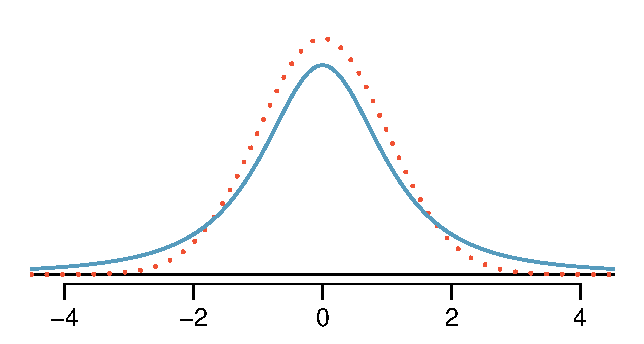
\includegraphics[width=0.6\textwidth]{ch_inference_for_means/figures/tDistCompareToNormalDist/tDistCompareToNormalDist}
\caption{Comparison of a $t$ distribution (solid line) and a normal distribution (dotted line).}
\label{tDistCompareToNormalDist}
\end{figure}

The $t$ distribution, always centered at zero, has a single parameter: degrees of freedom. The \termsub{degrees of freedom (df)}{degrees of freedom (df)!$t$ distribution} describe the precise form of the bell-shaped $t$ distribution. Several $t$ distributions are shown in Figure~\ref{tDistConvergeToNormalDist}. When there are more degrees of freedom, the $t$~distribution looks very much like the standard normal distribution.

\begin{figure}[h]
\centering
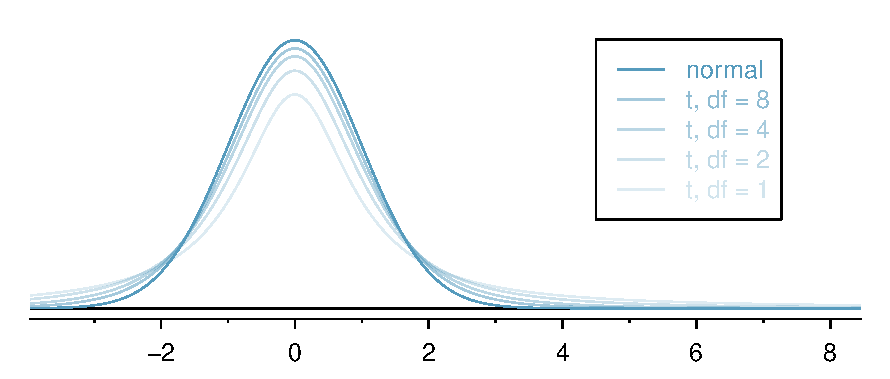
\includegraphics[width=0.9\textwidth]{ch_inference_for_means/figures/tDistConvergeToNormalDist/tDistConvergeToNormalDist}
\caption{The larger the degrees of freedom, the more closely the $t$ distribution resembles the standard normal model.}
\label{tDistConvergeToNormalDist}
\end{figure}

\begin{termBox}{\tBoxTitle{Degrees of freedom (df)}
The degrees of freedom describe the shape of the $t$ distribution. The larger the degrees of freedom, the more closely the distribution approximates the normal~model.}
\end{termBox}

When the degrees of freedom is about 30 or more, the $t$ distribution is nearly indistinguishable from the normal distribution. In Section~\ref{tDistSolutionToSEProblem}, we relate degrees of freedom to sample size.

We will find it very useful to become familiar with the $t$ distribution, because it plays a very similar role to the normal distribution during inference for numerical data. We use a \term{t table}, partially shown in Table~\ref{tTableSample}, in place of the normal probability table for numerical data when the population standard deviation is unknown, especially when the sample size is small. A~larger table is presented in Appendix~\ref{tDistributionTable}.

\begin{table}[hht]
\centering
\begin{tabular}{r | rrr rr}
one tail & \hspace{1.5mm}  0.100 & \hspace{1.5mm} 0.050 & \hspace{1.5mm} 0.025 & \hspace{1.5mm} 0.010 & \hspace{1.5mm} 0.005  \\
\hline
{$df$} \hfill 1  &  {\normalsize  3.078} & {\normalsize  6.314} & {\normalsize 12.71} & {\normalsize 31.82} & {\normalsize 63.66}  \\
2  &  {\normalsize  1.886} & {\normalsize  2.920} & {\normalsize  4.303} & {\normalsize  6.965} & {\normalsize  9.925}  \\
3  &  {\normalsize  1.638} & {\normalsize  2.353} & {\normalsize  3.182} & {\normalsize  4.541} & {\normalsize  5.841}  \\
$\vdots$ & $\vdots$ &$\vdots$ &$\vdots$ &$\vdots$ & \\
17  &  {\normalsize  1.333} & {\normalsize  1.740} & {\normalsize  2.110} & {\normalsize  2.567} & {\normalsize  2.898}  \\
\highlightO{18}  &  \highlightO{\normalsize  1.330} & \highlightO{\normalsize  1.734} & \highlightO{\normalsize  2.101} & \highlightO{\normalsize  2.552} & \highlightO{\normalsize  2.878}  \\
19  &  {\normalsize  1.328} & {\normalsize  1.729} & {\normalsize  2.093} & {\normalsize  2.539} & {\normalsize  2.861}  \\
20  &  {\normalsize  1.325} & {\normalsize  1.725} & {\normalsize  2.086} & {\normalsize  2.528} & {\normalsize  2.845}  \\
$\vdots$ & $\vdots$ &$\vdots$ &$\vdots$ &$\vdots$ & \\
1000  &  {\normalsize  1.282} & {\normalsize  1.646} & {\normalsize  1.962} & {\normalsize  2.330} & {\normalsize  2.581}  \\
$\infty$   &  {\normalsize  1.282} & {\normalsize  1.645} & {\normalsize  1.960} & {\normalsize  2.326} & {\normalsize  2.576}   \\
\hline
Confidence level C  &  {\normalsize  80\%} & {\normalsize 90\%} & {\normalsize 95\%} & {\normalsize  98\%} & {\normalsize  99\%}  \\
\hline
\end{tabular}
\caption{An abbreviated look at the $t$ table. Each row represents a different $t$ distribution. The columns describe the cutoffs for specific tail areas. The row with $df=18$ has been \highlightO{highlighted}.}
\label{tTableSample}
\end{table}

Each row in the $t$ table represents a $t$ distribution with different degrees of freedom. The columns correspond to tail probabilities. For instance, if we know we are working with the $t$ distribution with $df=18$, we can examine row 18, which is \highlightO{highlighted} in Table~\ref{tTableSample}. If we want the value in this row that identifies the cutoff for an upper tail of 10\%, we can look in the column where \emph{one tail} is 0.100. This cutoff is 1.33. If we had wanted the cutoff for the lower 10\%, we would use -1.33. Just like the normal distribution, all $t$ distributions are symmetric.

\textPE{\pagebreak}

\begin{example}{What proportion of the $t$ distribution with 18 degrees of freedom falls below -2.10?}
Just like a normal probability problem, we first draw the picture in Figure~\ref{tDistDF18LeftTail2Point10} and shade the area below -2.10. To find this area, we identify the appropriate row: $df=18$. Then we identify the column containing the absolute value of -2.10; it is the third column. Because we are looking for just one tail, we examine the top line of the table, which shows that a one tail area for a value in the third row corresponds to 0.025. About 2.5\% of the distribution falls below -2.10. In the next example we encounter a case where the exact $t$ value is not listed in the table.
\end{example}

\begin{figure}
\centering
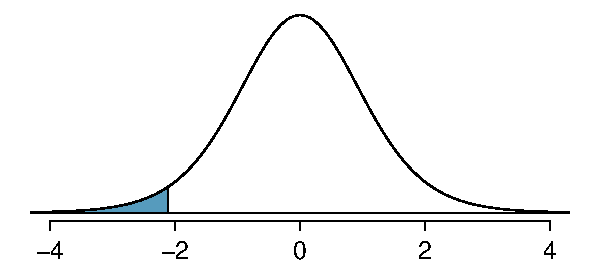
\includegraphics[width=0.6\textwidth]{ch_inference_for_means/figures/tDistDF18LeftTail2Point10/tDistDF18LeftTail2Point10}
\caption{The $t$ distribution with 18 degrees of freedom. The area below -2.10 has been shaded.}
\label{tDistDF18LeftTail2Point10}
\end{figure}

\textB{\pagebreak}

\begin{example}{A $t$ distribution with 20 degrees of freedom is shown in the left panel of Figure~\ref{tDistDF20RightTail1Point65}. Estimate the proportion of the distribution falling above 1.65.}
We identify the row in the $t$ table using the degrees of freedom: $df=20$. Then we look for 1.65; it is not listed. It falls between the first and second columns. Since these values bound 1.65, their tail areas will bound the tail area corresponding to 1.65. We identify the one tail area of the first and second columns, 0.050 and 0.10, and we conclude that between 5\% and 10\% of the distribution is more than 1.65 standard deviations above the mean. If we like, we can identify the precise area using statistical software: 0.0573.
\end{example}

\begin{figure}
\centering
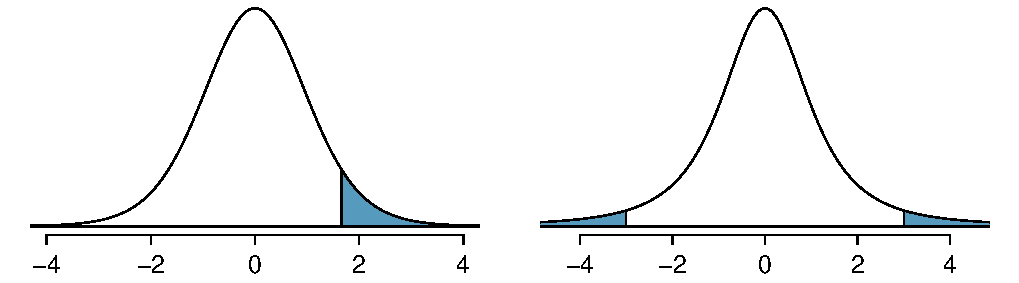
\includegraphics[width=0.96\textwidth]{ch_inference_for_means/figures/tDistDF20RightTail1Point65/tDistDF20RightTail1Point65}
\caption{Left: The $t$ distribution with 20 degrees of freedom, with the area above 1.65 shaded. Right: The $t$ distribution with 2 degrees of freedom, with the area further than 3 units from 0 shaded.}
\label{tDistDF20RightTail1Point65}
\end{figure}

\begin{example}{A $t$ distribution with 2 degrees of freedom is shown in the right panel of Figure~\ref{tDistDF20RightTail1Point65}. Estimate the proportion of the distribution falling more than 3 units from the mean (above or below).}
As before, first identify the appropriate row: $df=2$. Next, find the columns that capture 3; because $2.92 < 3 < 4.30$, we use the second and third columns. Finally, we find bounds for the tail areas by looking at the two tail values: 0.05 and 0.10. We use the two tail values because we are looking for two (symmetric) tails.
\end{example}


\subsection{The $t$ distribution and the standard error of a mean}
\label{tDistSolutionToSEProblem}

When estimating the mean and standard deviation from a small sample, the $t$ distribution is a more accurate tool than the normal model. This is true for both small and large samples.

\begin{tipBox}{\tipBoxTitle{When to use the $t$ distribution}
Use the $t$ distribution for inference of the sample mean when observations are independent and nearly normal. You may relax the nearly normal condition as the sample size increases. For example, the data distribution may be moderately skewed when the sample size is at least~30.
}
\end{tipBox}

\index{data!dolphins and mercury|(}

\textPE{\pagebreak}

%\CommentA{added n at least 30}
To proceed with the $t$ distribution for inference about a single mean, we must check two conditions.
\begin{description}
\setlength{\itemsep}{0mm}
\item[Independence of observations.] We verify this condition just as we did before. We collect a simple random sample from less than 10\% of the population, or if it was an experiment or random process, we carefully check to the best of our abilities that the observations were independent.
\item[$\mathbf{n\ge 30}$ or observations come from a nearly normal distribution.] We can easily check if the sample size is at least 30. If it is not, then this second condition requires more care. We often (i) take a look at a graph of the data, such as a dot plot or box plot, for obvious departures from the normal model, and (ii) consider whether any previous experiences alert us that the data may not be nearly normal.
\end{description}
When examining a sample mean and estimated standard deviation from a sample of $n$ independent and nearly normal observations, we use a $t$ distribution with $n-1$ degrees of freedom~($df$). For example, if the sample size was 19, then we would use the $t$ distribution with $df=19-1=18$ degrees of freedom and proceed exactly as we did in Chapter~\ref{foundationsForInference}, except that \emph{now we use the $t$ table}.

\begin{termBox}{\tBoxTitle{The t distribution and the SE of a mean}
In general, when the population mean is uknown, the population standard deviation will also be unknown. When this is the case, we estimate the population standard deviation with the sample standard deviation and we use SE instead of~SD.
\begin{align*}
SE_{\bar{x}}=\frac{s}{\sqrt{n}}
\end{align*}
When we use the sample standard deviation, we use the $t$ distribution with $df=n-1$ degrees of freedom instead of the normal distribution.}
\end{termBox}

\subsection{The normality condition}
\label{normalityCond}

When the sample size $n$ is at least 30, the Central Limit Theorem tells us that we do not have to worry too much about skew in the data. When this is not true, we need verify that the observations come from a nearly normal distribution. In some cases, this may be known, such as if the population is the heights of adults.

What do we do, though, if the population is not known to be approximately normal AND the sample size is small?  We must look at the distribution of the data and check for excessive skew.

\begin{caution}
{Checking the normality condition}
{We should exercise caution when verifying the normality condition for small samples. It is important to not only examine the data but also think about where the data come from. For example, ask: would I expect this distribution to be symmetric, and am I confident that outliers are rare?}
\end{caution}

You may relax the normality condition as the sample size goes up. If the sample size is~10 or more, slight skew is not problematic. Once the sample size hits about~30, then moderate skew is reasonable. Data with strong skew or outliers require a more \mbox{cautious analysis.}


\subsection{One sample $t$ confidence intervals}
\label{oneSampleTConfidenceIntervals}

Dolphins are at the top of the oceanic food chain, which causes dangerous substances such as mercury to concentrate in their organs and muscles. This is an important problem for both dolphins and other animals, like humans, who occasionally eat them. For instance, this is particularly relevant in Japan where school meals have included dolphin at times.
\setlength{\captionwidth}{71.5mm}

\begin{figure}[h]
\centering
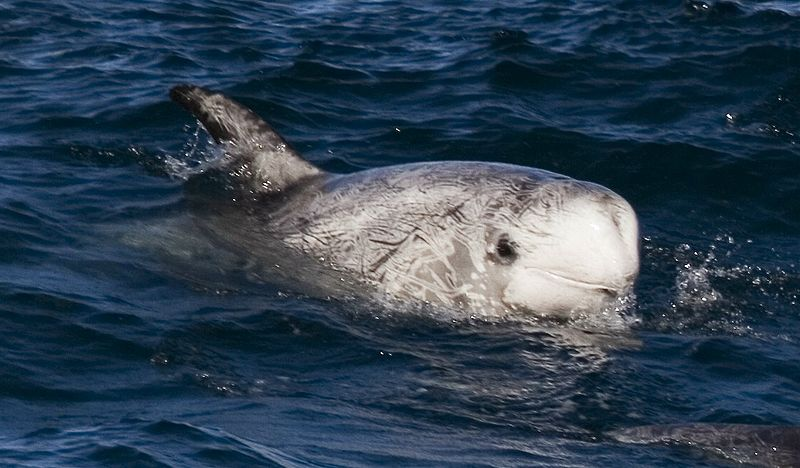
\includegraphics[width=0.7\textwidth]{ch_inference_for_means/figures/rissosDolphin/rissosDolphin.jpg}  \\
\addvspace{2mm}
\begin{minipage}{\textwidth}
   \caption[rissosDolphinPic]{A Risso's dolphin.\vspace{-1mm} \\
   -----------------------------\vspace{-2mm}\\
   {\footnotesize Photo by Mike Baird (\urlwofont{http://www.bairdphotos.com/}).%Image is under Creative Commons Attribution 2.0 Generic.
}\vspace{-8mm}}
   \label{rissosDolphin}
\end{minipage}
\vspace{3mm}
\end{figure}
\setlength{\captionwidth}{\mycaptionwidth}

Here we identify a confidence interval for the average mercury content in dolphin muscle using a sample of 19 Risso's dolphins from the Taiji area in Japan.\footnote{Taiji was featured in the movie \emph{The Cove}, and it is a significant source of dolphin and whale meat in Japan. Thousands of dolphins pass through the Taiji area annually, and we will assume these 19 dolphins represent a simple random sample from those dolphins. Data reference: Endo T and Haraguchi K. 2009. High mercury levels in hair samples from residents of Taiji, a Japanese whaling town. Marine Pollution Bulletin 60(5):743-747.} The data are summarized in Table~\ref{summaryStatsOfHgInMuscleOfRissosDolphins}. The minimum and maximum observed values can be used to evaluate whether or not there are obvious outliers or skew.

\begin{table}[h]
\centering
\begin{tabular}{ccc cc}
\hline
$n$ & $\bar{x}$ & $s$ & minimum & maximum \\
19   & 4.4	  & 2.3  & 1.7	       & 9.2 \\
\hline
\end{tabular}
\caption{Summary of mercury content in the muscle of 19 Risso's dolphins from the Taiji area. Measurements are in $\mu$g/wet g (micrograms of mercury per wet gram of muscle).}
\label{summaryStatsOfHgInMuscleOfRissosDolphins}
\end{table}

\begin{example}{Are the independence and normality conditions satisfied for this data~set?}
The observations are a simple random sample and consist of less than 10\% of the population, therefore independence is reasonable. The summary statistics in Table~\ref{summaryStatsOfHgInMuscleOfRissosDolphins} do not suggest any skew or outliers; all observations are within 2.5 standard deviations of the mean. Based on this evidence, the normality assumption seems reasonable.
\end{example}

In the normal model, we used $z^{\star}$ and the standard deviation to determine the width of a confidence interval. We revise the confidence interval formula slightly when using the $t$ distribution:
\begin{eqnarray*}
\bar{x} \ \pm\  t^{\star}_{df}SE
\end{eqnarray*}
\marginpar[\raggedright\vspace{-9mm}

$t^{\star}_{df}$\vspace{1mm}\\\footnotesize Multiplication\\factor for\\$t$ conf. interval]{\raggedright\vspace{-9mm}

$t^{\star}_{df}$\vspace{1mm}\\\footnotesize Multiplication\\factor for\\$t$ conf. interval}The sample mean is computed just as before: $\bar{x} = 4.4$. In place of the standard deviation of $\bar{x}$, we use the standard error of $\bar{x}$: $SE_{\bar{x}} = s/\sqrt{n} = 0.528$.

The value $t^{\star}_{df}$ is a cutoff we obtain based on the confidence level and the $t$ distribution with $df$ degrees of freedom. Before determining this cutoff, we will first need the degrees of freedom.

\begin{termBox}{\tBoxTitle{Degrees of freedom for a single sample}
If the sample has $n$ observations and we are examining a single mean, then we use the $t$ distribution with $df=n-1$ degrees of freedom.}
\end{termBox}

In our current example, we should use the $t$ distribution with $df=19-1=18$ degrees of freedom. Then identifying $t_{18}^{\star}$ is similar to how we found $z^{\star}$.
\begin{itemize}
\setlength{\itemsep}{0mm}
\item For a 95\% confidence interval, we want to find the cutoff $t^{\star}_{18}$ such that 95\% of the $t$ distribution is between -$t^{\star}_{18}$ and $t^{\star}_{18}$.
\item We look in the $t$ table on page~\pageref{tTableSample}, find the column with 95\% along the bottom row and then the row with 18 degrees of freedom: $t^{\star}_{18} = 2.10$.
\end{itemize}
Generally the value of $t^{\star}_{df}$ is slightly larger than what we would get under the normal model with~$z^{\star}$.

Finally, we can substitute all our values into the confidence interval equation to create the 95\% confidence interval for the average mercury content in muscles from Risso's dolphins that pass through the Taiji area:
\begin{align*}
\bar{x} \ &\pm\  t^{\star}_{18}SE  \\
4.4 \ &\pm\  2.10 \times 0.528 \quad df=18 \\
(3.29 &\text{ , } 5.51)
\end{align*}
We are 95\% confident the true average mercury content of muscles in Risso's dolphins is between 3.29 and 5.51 $\mu$g/wet gram. This is above the Japanese regulation level of 0.4 $\mu$g/wet gram.

\index{data!dolphins and mercury|)}

\begin{termBox}{\tBoxTitle{Finding a $t$ confidence interval for the mean}
Based on a sample of $n$ independent and nearly normal observations, a confidence interval for the population mean is
\begin{eqnarray*}
\bar{x} \ \pm\  t^{\star}_{df}SE \quad \quad df=n-1
\end{eqnarray*}
where $\bar{x}$ is the sample mean, $t^{\star}_{df}$ corresponds to the confidence level and degrees of freedom, and $SE$ is the standard error as estimated by the sample.}
\end{termBox}


\begin{termBox}{\tBoxTitle[]{Constructing a confidence interval for a mean}\vspace{-1mm}
\begin{enumerate}
\setlength{\itemsep}{0mm}
\item State the name of the CI being used: 1-sample t interval.
\item Verify conditions.\vspace{-1.5mm}
\begin{itemize}
\setlength{\itemsep}{0mm}
\item A simple random sample
\item Population is known to be normal OR $n\ge 30$ OR graph of sample is approximately symmetric with no outliers, making the assumption that the population is normal a reasonable one
\end{itemize}
\item Plug in the numbers and write the interval in the form
$$\text{point estimate } \pm \text{ critical value}\times \text{SE of estimate}$$
Use a point estimate of $\bar{x}$, $df = n-1$, find critical value $t^\star$ using the t table at row$=n-1$, and compute $SE = \frac{s}{\sqrt{n}}$.
\item Evaluate the CI and write in the form ( $\_$ , $\_$ ).
\item Interpret the interval:  ``We are [XX]\% confident that the true average of [...] is between [...] and [...]."
\item State your conclusion to the original question.
\end{enumerate}}
\end{termBox}

\begin{exercise} \label{croakerWhiteFishPacificExerConditions}
\index{data!white fish and mercury|(}
The FDA's webpage provides some data on mercury content of fish.\footnote{\urlwofont{http://www.fda.gov/food/foodborneillnesscontaminants/metals/ucm115644.htm}} Based on a sample of 15 croaker white fish (Pacific), a sample mean and standard deviation were computed as 0.287 and 0.069 ppm (parts per million), respectively. The 15 observations ranged from 0.18 to 0.41 ppm. We will assume these observations are independent. Construct an appropriate 95\% confidence interval for the true average mercury content of croaker white fish (Pacific). Is there evidence that the average mercury content is greater than 0.275 ppm?\footnote{The interval called for in this problem is a 1-sample t interval. We will assume that the sample was random. $n$ is small, but there are no obvious outliers; all observations are within 2 standard deviations of the mean. If there is skew, it is not evident. Therefore we do not have reason to believe the mercury content in the population is not nearly normal in this type of fish. We can now identify and calculate the necessary quantities. The point estimate is the sample average, which is 0.287.
The standard error: $SE = \frac{0.069}{\sqrt{15}} = 0.0178$. Degrees of freedom: $df = n - 1 = 14$. Using the t table, we identify $t^{\star}_{14} = 2.145$.
The confidence interval is given by: $0.287 \ \pm\  2.145\times 0.0178\ \to\ (0.249, 0.325)$. We are 95\% confident that the true average mercury content of croaker white fish (Pacific) is between 0.249 and 0.325 ppm. Because the interval contains 0.275 as well as value less than 0.275, we do not have evidence that the true \emph{average} mercury content is  greater than 0.275, even though our sample average was 0.287.}
\end{exercise}


\subsection{Choosing a sample size when estimating a mean}
\label{findingASampleSizeForACertainME}

\index{margin of error|(}

Many companies are concerned about rising healthcare costs. A company may estimate certain health characteristics of its employees, such as blood pressure, to project its future cost obligations. However, it might be too expensive to measure the blood pressure of every employee at a large company, and the company may choose to take a sample instead.

\textPE{\pagebreak}

\begin{example}{Blood pressure oscillates with the beating of the heart, and the systolic pressure is defined as the peak pressure when a person is at rest. The average systolic blood pressure for people in the U.S. is about 130 mmHg with a standard deviation of about 25 mmHg. How large of a sample is necessary to estimate the average systolic blood pressure with a margin of error of 4 mmHg using a 95\% confidence level?}
\label{sampleSizeComputationForSystolicBloodPressure}
First, we frame the problem carefully. Recall that the margin of error is the part we add and subtract from the point estimate when computing a confidence interval. When the standard deviation is known, the margin of error for a 95\% confidence interval estimating a mean can be written as
\begin{align*}
ME_{95\%} = 1.96\times\frac{\sigma_{employee}}{\sqrt{n}}
\end{align*}
The challenge in this case is to find the sample size $n$ so that this margin of error is less than or equal to 4, which we write as an inequality:
\begin{align*}
1.96\times \frac{\sigma_{employee}}{\sqrt{n}} \leq 4
\end{align*}
In the above equation we wish to solve for the appropriate value of $n$, but we need a value for $\sigma_{employee}$ before we can proceed. However, we haven't yet collected any data, so we have no direct estimate! Instead, we use the best estimate available to~us: the approximate standard deviation for the U.S. population, 25. To proceed and solve for $n$, we substitute 25 for $\sigma_{employee}$:
\begin{align*}
1.96\times \frac{\sigma_{employee}}{\sqrt{n}} \approx 1.96\times\frac{25}{\sqrt{n}}
	&\leq 4 \\
1.96\times\frac{25}{4} &\leq \sqrt{n} \\
\left(1.96\times\frac{25}{4}\right)^2 &\leq n \\
150.06 &\leq n \\
 n &= 151
\end{align*}
The minimum sample size that meets the condition is 151. We round up because the sample size must be an integer and it must be  \emph{greater than or equal to} 150.06.
\end{example}

A potentially controversial part of Example~\ref{sampleSizeComputationForSystolicBloodPressure} is the use of the U.S. standard deviation for the employee standard deviation. Usually the standard deviation is not known. In such cases, it is reasonable to review scientific literature or market research to make an educated guess about the standard deviation.

\begin{termBox}{\tBoxTitle{Identify a sample size for a particular margin of error}
To estimate the necessary sample size for a maximum margin of error $m$, we set up an equation to represent this relationship:
\begin{align*}
ME = z^{\star}\frac{\sigma}{\sqrt{n}} \leq m
\end{align*}
where $z^{\star}$ is chosen to correspond to the desired confidence level, and $\sigma$ is the standard deviation associated with the population. Solve for the sample size,~$n$.}
\end{termBox}

Sample size computations are helpful in planning data collection, and they require careful forethought. Next we consider another topic important in planning data collection and setting a sample size: the Type 2 Error rate.

\index{margin of error|)}



\subsection{Hypothesis testing for a mean}
\label{oneSampleTTests}

\index{data!SAT prep company|(}

%\CommentA{encountered major problem - this example actually uses paired data, which has not yet been discussed in this edition!!!  I am replacing it with example from ISRS and will use this example in the paired section.}
%CONSIDER: replacing the following application.

Is the typical US runner getting faster or slower over time? We consider this question in the context of the Cherry Blossom Run, comparing runners in 2006 and 2012. Technological advances in shoes, training, and diet might suggest runners would be faster in 2012. An opposing viewpoint might say that with the average body mass index on the rise, people tend to run slower. In fact, all of these components might be influencing run time.

The average time for all runners who finished the Cherry Blossom Run in 2006 was 93.29 minutes (93 minutes and about 17 seconds). We want to determine using data from 100 participants in the 2012 Cherry Blossom Run whether runners in this race are getting faster or slower, versus the other possibility that there has been no change.

\begin{exercise}
What are appropriate hypotheses for this context?\footnote{$H_0$: The average 10 mile run time in 2012 was the same as in 2006 (93.29 minutes). $\mu = 93.29$. $H_A$:~The average 10 mile run time for 2012 was \emph{different} than 93.29 minutes. $\mu \neq 93.29$.}
\end{exercise}

\begin{exercise}
The data come from a simple random sample from less than 10\% of all participants, so the observations are independent. However, should we be worried about skew in the data? A histogram of the differences was shown in the left panel of Figure~\ref{run10SampHistogramsInHTForMeanSubsection}.~\footnote{Since the sample size 100 is greater than 30, we do not need to worry about slight skew in the data.}
\end{exercise}

\begin{figure}
\centering
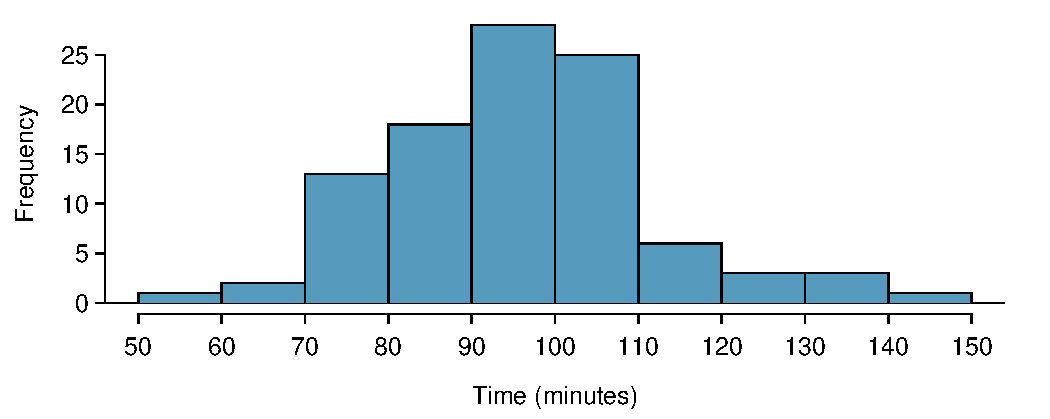
\includegraphics[width=0.77\textwidth]{ch_inference_for_means/figures/run10SampHistograms/run10SampHistograms} 
\caption{Histogram of \var{time} for a single sample of size 100.\index{skew!example: moderate}}
\label{run10SampHistogramsInHTForMeanSubsection}
\end{figure}

With independence satisfied and skew not a concern, we can proceed with performing a hypothesis test using the $t$ distribution.

\begin{exercise}
The sample mean and sample standard deviation are 95.61 and 15.78 minutes, respectively. Recall that the sample size is 100. What is the p-value for the test, and what is your conclusion?\footnote{With the conditions satisfied for the $t$ distribution, we can compute the standard error ($SE = 15.78 / \sqrt{100} = 1.58$ and the \emph{T score}: $T = \frac{95.61 - 93.29}{1.58} = 1.47$. For $df = 100 - 1 = 99$, we would find a p-value between 0.10 and 0.20 (two-sided!). Because the p-value is greater than 0.05, we do not reject the null hypothesis. That is, the data do not provide strong evidence that the average run time for the Cherry Blossom Run in 2012 is any different than the 2006 average.}
\end{exercise}

\begin{termBox}{\tBoxTitle[]{Hypothesis test for a mean}
\begin{enumerate}
\setlength{\itemsep}{0mm}
\item State the name of the test being used: 1-sample t test.
\item Verify conditions.\vspace{-1.5mm}
\begin{itemize}
\setlength{\itemsep}{0mm}
\item Data come from a simple random sample.
\item Population is known to be normal OR $n\ge 30$ OR graph of data is approximately symmetric with no outliers, making the assumption that population is normal a reasonable one.
\end{itemize}
\item Write the hypotheses in plain language, then set them up in mathematical notation.\vspace{-1.5mm}
\begin{itemize}
\setlength{\itemsep}{0mm}
\item H$_0: \mu = \mu_0$
\item H$_0: \mu \ne \text{or} < \text{or} > \mu_0$
\end{itemize}
\item Identify the significance level $\alpha$.
\item Calculate the test statistic and $df$.
$$\text{t} = \frac{\text{point estimate} - \text{null value}}{\text{SE of estimate}}$$
The point estimate is $\bar{x}$, $SE = \frac{s}{\sqrt{n}}$, and $df=n-1$.
\item Find the p-value, compare it to $\alpha$, and state whether to reject or not reject the null hypothesis.
\item Write your conclusion.
\end{enumerate}}
\end{termBox}

\begin{exercise}Recall the example about the mercury content in croaker white fish (Pacific). Based on a sample of 15, a sample mean and standard deviation were computed as 0.287 and 0.069 ppm (parts per million), respectively. Carry out an appropriate test to determine 0.25 is a reasonable value for the average mercury content.\footnote{We should carry out a 1-sample t test. The conditions have already been checked. $H_0: \mu=0.25$; The true average mercury content is 0.25 ppm. $H_A: \mu \ne 0.25$; The true average mercury content is not equal to 0.25 ppm. Let $\alpha=0.05$. $SE = \frac{0.069}{\sqrt{15}} = 0.0178$. $t=\frac{0.287-0.25}{0.0178}=2.07$  $df=15-1=14$. p-value$=0.057>0.05$, so we do not reject the null hypothesis. We do not have sufficient evidence that the average mercury content in croaker white fish is not 0.25.}
\end{exercise}

%\CommentA{for the next edition, this example should be put sooner and in the context of proportions. thought of that after I had already written this.}

\begin{example}{Recall that the 95\% confidence interval for the average mercuy content in croaker white fish was (0.249, 0.325). Discuss whether the conclusion of the test of hypothesis is consistent or inconsistent with the conclusion of the hypothesis test.}It is consistent because 0.25 is located (just barely) inside the confidence interval, so it is a reasonable value. Our hypothesis test did not reject the hypothesis that $\mu=0.25$, implying that it is a plausible value. Note, though, that the hypothesis test did not \emph{prove} that $\mu=.25$. A hypothesis cannot prove that the mean is a specific value. It can only find evidence that it is not a specific value. Note also that the p-value was close to the cutoff of 0.05. This is because the value 0.25 was close to edge of the confidence interval.
\end{example}

\subsection{Calculator: The 1-sample t test and CI}

\begin{termBox}{\tBoxTitle{TI calculator: Carrying out the 1-sample t test}
Use \textbf{STAT, TESTS, T-Test}.
\begin{enumerate}
\setlength{\itemsep}{0mm}
\item Choose STAT.
\item Right arrow to TESTS.
\item Down arrow and choose 2: T-Test.
\item Choose Data if you have all the data or Stats if you have the mean and standard deviation.
\item Let $\mu_0$ be the null or hypothesized value of $\mu$.
\begin{itemize}
\item If you choose Data, let List be L1 or the list in which you entered your data (don't forget to enter the data!) and let Freq be 1.
\item If you choose Stats, enter the mean, SD, and sample size.
\end{itemize}
\item Choose $\ne$, $<$, or $>$ to correspond to H$_A$.
\item Choose Calculate and hit ENTER, which returns: \\
\begin{tabular}{l l}
\text{t} &\quad \text{t statistic} \\
\text{p} &\quad \text{p-value} \\
$\bar{x}$ &\quad \text{the sample mean} \\
\text{Sx} &\quad \text{the sample SD} \\
\text{n} &\quad \text{the sample size}
\end{tabular}
\end{enumerate}
}
\end{termBox}

\begin{termBox}{\tBoxTitle{TI calculator: Calculating the 1-sample t Confidence Interval}
Use \textbf{STAT, TESTS, TInterval}.
\begin{enumerate}
\setlength{\itemsep}{0mm}
\item Choose STAT.
\item Right arrow to TESTS.
\item Down arrow and choose 8: TInterval.
\item Choose Data if you have all the data or Stats if you have the mean and standard deviation.
\begin{itemize}
\item If you choose Data, let List be L1 or the list in which you entered your data (don't forget to enter the data!) and let Freq be 1.
\item If you choose Stats, enter the mean, SD, and sample size.
\end{itemize}
\item Let C-Level be the desired confidence level.
\item Choose Calculate and hit ENTER, which returns:\\
\begin{tabular}{l l}
\text{( $\_$ , $\_$ )} &\quad \text{the confidence interval} \\
$\bar{x}$ &\quad \text{the sample mean} \\
\text{Sx} &\quad \text{the sample SD} \\
\text{n} &\quad \text{the sample size}
\end{tabular}
\end{enumerate}
}
\end{termBox}

\textPE{\pagebreak}

\begin{exercise}In the previous example, we saw that an SAT prep company claimed that they improve students' scores by 100 points. A sample of size 30 students that used the company produced a mean 135.9 and standard deviation 82.2. Use a calculator to find the t statistic and the p-value.\footnote{Choose Stats and let $\mu_0$ be 100. Choose $>$ to correspond to $H_A$. $t=2.39$ and p-value$=0.012$.}
\end{exercise}

\begin{exercise}Use a calculator to find a 95\% confidence interval for the true improvement of students that use this SAT prep company.\footnote{The interval is $(105.21, 166.59)$.}
\end{exercise}

%__________________
\section{Inference for paired data}
\label{pairedData}


\index{paired data|(}
\index{data!textbooks|(}

%\Comment{moved matched pairs section here and redid using t}

Are textbooks actually cheaper online? Here we compare the price of textbooks at UCLA's bookstore and prices at Amazon.com. Seventy-three UCLA courses were randomly sampled in Spring 2010, representing less than 10\% of all UCLA courses.\footnote{When a class had multiple books, only the most expensive text was considered.} A portion of this data set is shown in Table~\ref{textbooksDF}.

\begin{table}[h]
\centering
\begin{tabular}{rllrrr}
  \hline
 & dept & course & ucla & amazon & diff \\
  \hline
1 & Am Ind &  C170 & 27.67 & 27.95 & -0.28 \\
  2 & Anthro & 9 & 40.59 & 31.14 & 9.45 \\
  3 & Anthro & 135T & 31.68 & 32.00 & -0.32 \\
  4 & Anthro & 191HB & 16.00 & 11.52 & 4.48 \\
$\vdots$ & $\vdots$ & $\vdots$ & $\vdots$ & $\vdots$ & $\vdots$ \\
  72 & Wom Std & M144 & 23.76 & 18.72 & 5.04 \\
  73 & Wom Std & 285 & 27.70 & 18.22 & 9.48 \\
   \hline
\end{tabular}
\caption{Six cases of the \data{textbooks} data set.}
\label{textbooksDF}
\end{table}
%library(openintro); library(xtable); data(textbooks); xtable(textbooks[c(1:5, nrow(textbooks) - 1:0),])

\subsection{Paired observations and samples}

Each textbook has two corresponding prices in the data set: one for the UCLA bookstore and one for Amazon. Therefore, each textbook price from the UCLA bookstore has a natural correspondence with a textbook price from Amazon. When two sets of observations have this special correspondence, they are said to be \term{paired}.

\begin{termBox}{\tBoxTitle{Paired data}
Two sets of observations are \emph{paired} if each observation in one set has a special correspondence or connection with exactly one observation in the other data set.}
\end{termBox}

To analyze paired data, it is often useful to look at the difference in outcomes of each pair of observations. In the \data{textbook} data set, we look at the difference in prices, which is represented as the \var{diff} variable in the \data{textbooks} data. Here the differences are taken as
\begin{eqnarray*}
\text{UCLA price} - \text{Amazon price}
\end{eqnarray*}
for each book. It is important that we always subtract using a consistent order; here Amazon prices are always subtracted from UCLA prices. If this difference is positive, the UCLA price is higher. If ths difference is negative, the Amazon price is higher. If this difference is zero, the two prices are equal. A histogram of these differences is shown in Figure~\ref{diffInTextbookPricesS10}. Using differences between paired observations is a common and useful way to analyze paired data.

\begin{figure}
\centering
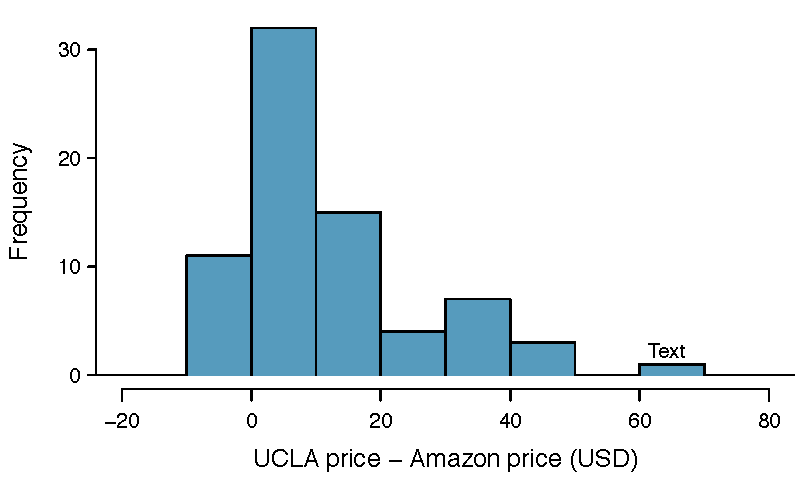
\includegraphics[width=0.83\textwidth]{ch_inference_for_means/figures/textbooksS10/diffInTextbookPricesS10}
\caption{Histogram of the difference in price for each of the 73 books sampled. These data are strongly skewed.\index{skew!example: strong}}
\label{diffInTextbookPricesS10}
\end{figure}

\begin{exercise}
The first difference shown in Table~\ref{textbooksDF} is computed as $27.67-27.95=-0.28$. Verify the differences are calculated correctly for observations 2 and 3.\footnote{Observation 2: $40.59 - 31.14 = 9.45$. Observation 3: $31.68 - 32.00 = -0.32$.}
\end{exercise}

\subsection{Hypothesis testing for paired data}

To analyze a paired data set, we use the exact same tools that we developed in the previous section. Now we apply them to the differences in the paired observations.

\begin{table}[hh]
\centering
\begin{tabular}{ccccc}
\hline
$n_{_{diff}}$	&\hspace{3mm}& $\bar{x}_{_{diff}}$	&\hspace{3mm}& $s_{_{diff}}$ \vspace{1mm}\\
73			&& 12.76				&& 14.26 \\
\hline
\end{tabular}
\caption{Summary statistics for the price differences. There were 73 books, so there are 73 differences.}
\label{textbooksSummaryStats}
\end{table}

\begin{example}{Set up and implement a hypothesis test to determine whether, on average, there is a difference between Amazon's price for a book and the UCLA bookstore's price.}
\label{htForDiffInUCLAAndAmazonTextbookPrices}
There are two scenarios: there is no difference or there is some difference in average prices. The \emph{no difference} scenario is always the null hypothesis:
\begin{itemize}
\setlength{\itemsep}{0mm}
\item[$H_0$:] $\mu_{diff}=0$. There is no difference in the average textbook price.
\item[$H_A$:] $\mu_{diff} \neq 0$. There is a difference in average prices.
\end{itemize}
The standard deviation of all of the differences in unknown, so we will use the standard deviation of the sample differences. The observations are based on a simple random sample from less than 10\% of all books sold at the bookstore, so independence is reasonable; the distribution of differences, shown in Figure~\ref{diffInTextbookPricesS10}, is strongly skewed, but this amount of skew is reasonable for this sized data set ($n=73$). Because all three conditions are reasonably satisfied, we can conclude the t test is reasonable.

We compute the standard error associated with $\bar{x}_{diff}$ using the standard deviation of the differences ($s_{_{diff}}=14.26$) and the number of differences ($n_{_{diff}}=73$):
$$SE_{\bar{x}_{diff}} = \frac{s_{diff}}{\sqrt{n_{diff}}} = \frac{14.26}{\sqrt{73}} = 1.67$$
To visualize the p-value, the sampling distribution of $\bar{x}_{diff}$ is drawn as though $H_0$ is true, which is shown in Figure~\ref{textbooksS10HTTails}. The p-value is represented by the two (very) small tails.

\begin{figure}
\centering
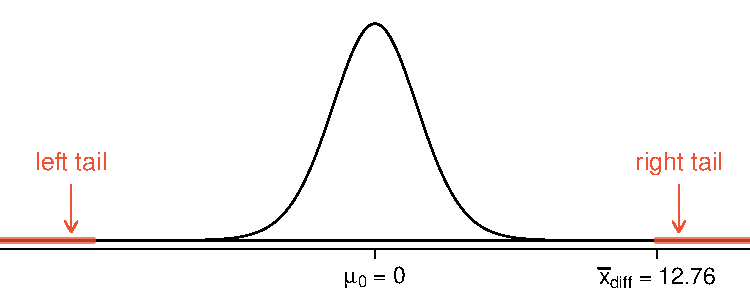
\includegraphics[width=0.65\textwidth]{ch_inference_for_means/figures/textbooksS10/textbooksS10HTTails}
\caption{Sampling distribution for the mean difference in book prices, if the true average difference is zero.}
\label{textbooksS10HTTails}
\end{figure}

To find the tail areas, we compute the test statistic, which is the t score of $\bar{x}_{diff}$ under the null condition that the actual mean difference is 0:
$$t = \frac{\bar{x}_{diff} - 0}{SE_{x_{diff}}} = \frac{12.76 - 0}{1.67} = 7.59  \quad \quad \quad df=72$$
This t score is so large it isn't even in the table, which ensures the single tail area will be 0.0002 or smaller. A calculator gives a tail area as $4.5\times 10^{-11}$. Since the p-value corresponds to both tails in this case and the $t$ distribution is symmetric, the p-value can be estimated as twice the one-tail area:
$$\text{p-value} = 2\times (\text{one tail area}) \approx 2\times 4.5\times 10^{-11} = 9\times 10^{-11}\approx 0$$
Because the p-value is less than 0.05, we reject the null hypothesis. We have found convincing evidence that Amazon is, on average, cheaper than the UCLA bookstore for UCLA course textbooks.
\end{example}

\begin{termBox}{\tBoxTitle[]{Hypothesis test for paired data}
\begin{enumerate}
\setlength{\itemsep}{0mm}
\item State the name of the test being used: matched pairs t test.
\item Verify conditions.\vspace{-1.5mm}
\begin{itemize}
\setlength{\itemsep}{0mm}
\item Paired data from a random sample or experiment
\item Population of differences is known to be normal OR $n_{diff}\ge 30$ OR graph of sample differences is approximately symmetric with no outliers, making the assumption that population of differences is normal a reasonable one
\end{itemize}
\item Write the hypotheses in plain language, then set them up in mathematical notation.\vspace{-1.5mm}
\begin{itemize}
\setlength{\itemsep}{0mm}
\item H$_0: \mu_{diff}=0$
\item H$_0: \mu_{diff} \ne \text{or} < \text{or} > 0$
\end{itemize}
\item Identify the significance level $\alpha$.
\item Calculate the test statistic and $df$.
$$\text{t} = \frac{\text{point estimate} - \text{null value}}{\text{SE of estimate}}$$
Where the point estimate is $\bar{x}_{diff}$, $SE = \frac{s_{diff}}{\sqrt{n_{diff}}}$, and $df=n_{diff}-1$.
\item Find the p-value and compare it to $\alpha$ to determine whether to reject or not reject $H_0$.
\item Write the conclusion in the context of the question.
\end{enumerate}}
\end{termBox}

\begin{figure}[h]
\centering
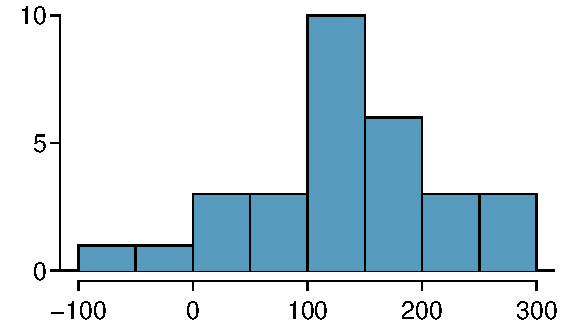
\includegraphics[width=0.54\textwidth]{ch_inference_for_means/figures/satImprovementHTDataHistogram/satImprovementHTDataHistogram}
\caption{Sample distribution of:  SAT score after course - SAT score before course. The distribution is approximately symmetric.}
\label{satImprovementHTDataHistogram}
\end{figure}

%\CommentA{please format footnote as you like}

\textPE{\newpage}

\begin{exercise}An SAT preparation company claims that its students' scores improve by over 100 points on average after their course. A consumer group would like to evaluate this claim, and they collect data on a random sample of 30 students who took the class. Each of these students took the SAT before and after taking the company's course, and so we have a difference in scores for each student. We will examine these differences $x_1=57$, $x_2=133$, ..., $x_{30}=140$ as a sample to evaluate the company's claim. The distribution of the differences, shown in Figure~\ref{satImprovementHTDataHistogram}, has mean 135.9 and standard deviation 82.2. Do these data provide convincing evidence to back up the company's claim?
\footnote{This is \emph{paired data}, so we analyze the score differences with a matched pairs t test. Conditions: This is a random sample from less than 10\% of the company's students (assuming they have more than 300 former students), so the independence condition is reasonable. $n=30\ge 30$.
This is a one-sided test. $H_0$: student scores do not improve by more than 100 after taking the company's course. $\mu_{_{diff}} = 100$  $H_A$: students scores improve by more than 100 points on average after taking the company's course. $\mu_{_{diff}} > 100$.
Let
\begin{align*}
\alpha&=0.05
&&SE = \frac{82.2}{\sqrt{30}} = 15.0
&&T = \frac{135.9-100}{15.0}=2.4
&&\text{with }df=29
\end{align*}
p-value$=0.012<\alpha$ so we reject the null hypothesis. The data provide convincing evidence to support the company's claim that student scores improve by more than 100 points following the class.}
\end{exercise}

\begin{exercise}
Because we rejected the null hypothesis, does this mean that taking the company's class improves student scores by more than 100 points on average?\footnote{This is an observational study, so we cannot make this causal conclusion. For instance, maybe SAT test takers tend to improve their score over time even if they don't take a special SAT class, or perhaps only the most motivated students take such SAT courses.}

\index{data!SAT prep company|)}

\end{exercise}



\subsection{Confidence intervals for the mean of a difference $\mu_{1-2}$}

\begin{exercise}
Create a 95\% confidence interval for the average price difference between books at the UCLA bookstore and books on Amazon.\footnote{Conditions have already verified and the standard error computed in Example~\ref{htForDiffInUCLAAndAmazonTextbookPrices}. To find the interval, identify $t
^{\star}$ (round $df=72$ down to 60 to get a $t^{\star}$ of 2.00  for 95\% confidence) and plug it, the point estimate, and the standard error into the confidence interval formula:
\begin{align*}
\text{point estimate} \ &\pm\ t^{\star}SE \quad \quad \quad \quad df=n-1\\
12.76 \ &\pm\ 2.00\times 1.67 \quad \quad  df=72\\
(9.42 &\text{ , } 16.10)
\end{align*}
We are 95\% confident that Amazon is, on average, between \$9.42 and \$16.10 cheaper than the UCLA bookstore for UCLA course books.}

\index{data!textbooks|)}
\index{paired data|)}

\end{exercise}

\textPE{\newpage}

\begin{termBox}{\tBoxTitle[]{Constructing a confidence interval for paired data}\vspace{-1mm}
\begin{enumerate}
\setlength{\itemsep}{0mm}
\item State the name of the CI being used: matched pairs t interval.
\item Verify conditions.\vspace{-1.5mm}
\begin{itemize}
\setlength{\itemsep}{0mm}
\item Paired data from a random sample or experiment
\item Population of diferrences is known to be normal OR $n_{diff}\ge 30$ OR graph of sample differences is approximately symmetric with no outliers, making the assumption that the population of differences is normal a reasonable one
\end{itemize}
\item Plug in the numbers and write the interval in the form
$$\text{point estimate } \pm \text{ critical value}\times \text{SE of estimate}$$
Use the point estimate of $\bar{x}_{diff}$, $df=n_{diff}-1$, find critical value $t^\star$ using the t table at row $n_{diff}-1$, and compute the $SE = \frac{s_{diff}}{\sqrt{n_{diff}}}$.
\item Evaluate the CI and write in the form ( $\_$ , $\_$ ).
\item Interpret the interval: ``We are [XX]\% confident that the true mean of the difference in [...] is between [...] and [...]."
\item State your conclusion to the original question.
\end{enumerate}}
\end{termBox}

\begin{exercise}In the SAT preparation company example, we saw that $\bar{x}_{diff}$ was 135.9 and $s_{diff}$ was 82.2. That~is, the average change in students' scores after the class was a 135.9 point increase and the SD of the change or difference in their scores was 82.2 points. Construct a 95\% confidence interval to estimate the true average change in score after taking the class. Is there evidence for the company's claim that students score an average of 100 points higher after the class?\footnote{Because this is a before and after scenario, we use a matched pairs t interval. The conditions were verified in the previous section. The confidence interval is : $135.9\ \pm 2.045(15.0) \to (105.2, 166.6)$. We can be 95\% confident that the true \emph{average} increase in scores after the prep class is between 105.2 and 166.6. Because the entire interval is above 100, there is evidence that on average students score more than 100 points higher after the course. Recall that this does not prove that the increase is \emph{due to}  the course.}
\end{exercise}

\begin{exercise}The 95\% confidence interval in the previous exercise was calculated as (105.2, 166.6). True or false: about 9\% of the students that take the class will saw an increase of at least 105.2 points.\footnote{False. This confidence interval estimates the \emph{average} increase - not the increase of individuals. As can be seen in Figure~\ref{satImprovementHTDataHistogram}, much greater than 5\% saw an increase of less than 105.2 points. Some individuals even saw a \emph{decrease} in their score as indicated by the negative differences.}
\end{exercise}


\subsection{Calculator: the matched pairs t test and CI}

\begin{termBox}{\tBoxTitle{TI calculator: Carrying out the matched pairs t test}
Use \textbf{STAT, TESTS, T-Test}.
\begin{enumerate}
\setlength{\itemsep}{0mm}
\item Choose STAT.
\item Right arrow to TESTS.
\item Down arrow and choose 2: T-Test.
\item Choose Data if you have all the data or Stats if you have the mean and standard deviation.
\item Let $\mu_0$ be the null or hypothesized value of $\mu_{diff}$.
\begin{itemize}
\setlength{\itemsep}{0mm}
\item If you choose Data, let List be L3 or the list in which you entered the differences (don't forget to enter the differences!) and let Freq be 1.
\item If you choose Stats, enter the mean, SD, and sample size of the differences.
\end{itemize}
\item Choose $\ne$, $<$, or $>$ to correspond to H$_A$.
\item Choose Calculate and hit ENTER, which returns:
\begin{tabular}{l l}
\text{t} &\quad \text{t statistic} \\
\text{p} &\quad \text{p-value} \\
$\bar{x}$ &\quad \text{the sample mean of the differences} \\
\text{Sx} &\quad \text{the sample SD of the differences} \\
\text{n} &\quad \text{the sample size of the differences}
\end{tabular}
\end{enumerate}
}
\end{termBox}

\begin{termBox}{\tBoxTitle{TI calculator: Calculating the matched pairs t Confidence Interval}
Use \textbf{STAT, TESTS, TInterval}.
\begin{enumerate}
\setlength{\itemsep}{0mm}
\item Choose STAT.
\item Right arrow to TESTS.
\item Down arrow and choose 8: TInterval.
\item Choose Data if you have all the data or Stats if you have the mean and standard deviation.
\begin{itemize}
\item If you choose Data, let List be L3 or the list in which you entered the differences (don't forget to enter the differences!) and let Freq be 1.
\item If you choose Stats, enter the mean, SD, and sample size of the differences.
\end{itemize}
\item Let C-Level be the desired confidence level.
\item Choose Calculate and hit ENTER, which returns:
\begin{tabular}{l l}
\text{( $\_$ , $\_$ )} &\quad \text{the confidence interval for the differences} \\
$\bar{x}$ &\quad \text{the sample mean of the differences} \\
\text{Sx} &\quad \text{the sample SD of the differences} \\
\text{n} &\quad \text{the number of differences in the sample}
\end{tabular}
\end{enumerate}
}
\end{termBox}

\begin{table}[h]
\centering
\begin{tabular}{rlll}
  \hline
 & dept & ucla & amazon \\
  \hline
1 & Am Ind &   27.67 & 27.95 \\
  2 & Anthro &  40.59 & 31.14  \\
  3 & Anthro &  31.68 & 32.00  \\
  4 & Anthro &  16.00 & 11.52  \\
5 & Art His & 18.95 &14.21	\\
6 & Art His &14.95&	10.17	\\
7 & Asia Am &	24.7&	20.06	\\
   \hline
\end{tabular}
\caption{A partial table of the \data{textbooks} data.}
\label{textbooksDFPartial}
\end{table}

\begin{exercise}Use the first 7 values of the ~\ref{textbooksDF} data set produced above and calculate the t score and p-value to test whether, on average, Amazon's textbook price is cheaper that UCLA's price.\footnote{Enter the data into L1  and L2 on a calculator. Let $L3 = L1-L2$. After selecting TTest, choose DATA, let $\mu_0$ be 0, and let List be \textbf{L3}. Let Freq be 1 and  select $>$. $t=3.076$ and p-value$=0.0109$.}\end{exercise}

\begin{exercise}Use the first 7 values of the ~\ref{textbooksDF} data set produced above and calculate a 95\% confidence interval for the average difference in textbook price between Amazon and UCLA.\footnote{The data have already been entered into L1  and L2 and the differences should be in L3. After selecting TInterval, choose DATA, let List be \textbf{L3}. Let Freq be 1 and let C-Level be 0.95. The interval is (.80354, 7.0507).}\end{exercise}

%__________________
\section{Difference of two means using the $t$ distribution}
\label{theTDistributionForTheDifferenceOfTwoMeans}

It is also useful to be able to compare two means for small samples. For instance, a teacher might like to test the notion that two versions of an exam were equally difficult. She could do so by randomly assigning each version to students. If she found that the average scores on the exams were so different that we cannot write it off as chance, then she may want to award extra points to students who took the more difficult exam.

In a medical context, we might investigate whether embryonic stem cells can improve heart pumping capacity in individuals who have suffered a heart attack. We could look for evidence of greater heart health in the stem cell group against a control group.

In this section we use the $t$ distribution for the difference in sample means. We will again drop the minimum sample size condition and instead impose a strong condition on the distribution of the data.


\subsection{Sampling distribution for the difference of two means}
\label{differenceOfTwoMeans}

In this section we consider a difference in two population means, $\mu_1 - \mu_2$, under the condition that the data are not paired. The methods are similar in theory but different in the details. Just as with a single sample, we identify conditions to ensure a point estimate of the difference $\bar{x}_1 - \bar{x}_2$ is nearly normal. Next we introduce a formula for the standard deviation of $\bar{x}_1 - \bar{x}_2$, which allows us to apply our general tools from Section~\ref{foundationsForInference}.

We apply these methods to two examples: participants in the 2012 Cherry Blossom Run and newborn infants. This section is motivated by questions like ``Is there convincing evidence that newborns from mothers who smoke have a different average birth weight than newborns from mothers who don't smoke?''

\index{data!run10Samp|(}

\index{point estimate!difference of means|(}
We start by looking at the population mean and standard deviation  for the run times of men and women participants in the 2009 Cherry Blossom Run. Table~\ref{cherryBlossomRun2009SampleOf180SummaryStats} summarizes these values.

\begin{table}[h]
\centering
\begin{tabular}{l rr}
\hline
	&	men	&	women \\
\hline
$\mu$	& 87.65	& 102.13 \\
$\sigma$	&	12.5		& 15.2 \\
%$N$	&	45		& 55    \\
\hline
\end{tabular}
\caption{Summary of the run time of participants in the 2009 Cherry Blossom Run.}
\label{cherryBlossomRun2009SampleOf180SummaryStats}
\end{table}
%library(openintro); data(run10Samp); d <- run10Samp; by(d$time, d$gender, mean); by(d$time, d$gender, sd); by(d$time, d$gender, length)

% ALERT: marked as to be cut, but forgot to cut before formatting. Just leaving in.
\begin{figure}[h]
\centering
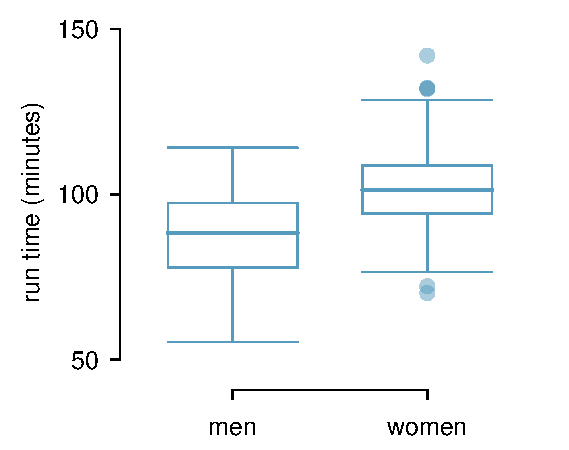
\includegraphics[width=0.5\textwidth]{ch_inference_for_means/figures/cbrRunTimesMenWomen/cbrRunTimesMenWomen}
\caption{Side-by-side box plots for the sample of 2009 Cherry Blossom Run participants.}
\label{cbrRunTimesMenWomen}
\end{figure}

The two populations (men and women) are independent of one-another, so the data are not paired.\footnote{Probability theory guarantees that the difference of two independent normal random variables is also normal. Because each sample mean is nearly normal and observations in the samples are independent, we are assured the difference is also nearly normal.} If we take two separate random samples of men and women from this race, what is the expected value for the difference in their average times? Not surprisingly, the expected value of $\bar{x}_{w} - \bar{x}_{m}$ is $\mu_1-\mu_2$. We can quantify the variability in the point estimate, using the following formula for its standard deviation:
\index{standard error!difference in means}
\begin{align*}
SD_{\bar{x}_{w} - \bar{x}_{m}}
    &= \sqrt{\left(SD_{\bar{x}_{w}}\right)^2 +\left(SD_{\bar{x}_{m}}\right)^2 } \\
    &= \sqrt{\left(\frac{\sigma_{\bar{x}_{w}}}{\sqrt{n_w}}\right)^2 + \left(\frac{\sigma_{\bar{x}_{m}}}{\sqrt{n_m}}\right)^2 } \\
	&= \sqrt{\frac{\sigma_{w}^2}{n_{w}} + \frac{\sigma_{m}^2}{n_{m}}} \\
\end{align*}
\begin{exercise}
Let's say we take a random sample of 55 women and a random sample of 45 men. Use the SD formula for the difference of two means to compute the SD for the difference in the average run time for males and females.\footnote{$\sqrt{\frac{15.2^2}{55} + \frac{12.5^2}{45}} = 2.77$}
\end{exercise}

\index{point estimate!difference of means|)}

\begin{termBox}{\tBoxTitle{Distribution of a difference of sample means}
The sample difference of two means, $\bar{x}_1 - \bar{x}_2$, is nearly normal with mean $\mu_{1}-\mu_{2}$ and standard deviation
\begin{eqnarray}
SD_{\bar{x}_{1} - \bar{x}_{2}} = \sqrt{\frac{\sigma_1^2}{n_1} + \frac{\sigma_2^2}{n_2}}
\label{seOfDifferenceInMeans}
\end{eqnarray}
when each sample mean is nearly normal and all observations are independent. Recall that each sample mean will be nearly normal if the population is normal or if the sample size is at least 30.}
\end{termBox}


%-
\subsection{Point estimates and standard errors for differences of means}
In the example of two exam versions, the teacher would like to evaluate whether there is convincing evidence that the difference in average scores between the two exams is not due to chance.

It will be useful to extend the $t$ distribution method from Section~\ref{oneSampleMeansWithTDistribution} to apply to a difference of means:
\begin{eqnarray*}
\bar{x}_1 - \bar{x}_2
	\qquad \text{as a point estimate for} \qquad
	\mu_1 - \mu_2
\end{eqnarray*}
First, we verify the small sample conditions (independence and nearly normal data) for each sample separately, then we verify that the samples are also independent. For instance, if the teacher believes students in her class are independent, the exam scores are nearly normal, and the students taking each version of the exam were independent, then we can use the $t$ distribution for inference on the point estimate $\bar{x}_{1} - \bar{x}_{2}$.

The formula for the standard error of $\bar{x}_{1} - \bar{x}_{2}$, introduced in Section~\ref{differenceOfTwoMeans},
also applies to small samples:
\begin{eqnarray}
SE_{\bar{x}_1 - \bar{x}_2}
	= \sqrt{SE_{\bar{x}_1}^2 + SE_{\bar{x}_2}^2}
	 = \sqrt{\frac{s_1^2}{n_1} + \frac{s_2^2}{n_2}} \label{seOfDiffOfTwoMeansInTDistSection}
\end{eqnarray}
Because we will use the $t$ distribution, we will need to identify the appropriate degrees of freedom. This can be done using a calculator or computer software. An alternative technique is to use the smaller of $n_1 - 1$ and $n_2 - 1$.~\footnote{This technique for degrees of freedom is conservative with respect to a Type 1 Error; it is more difficult to reject the null hypothesis using this $df$ method.}

%\Comment{In practice, students will always use calculator to find df for difference of two means.}

\begin{termBox}{\tBoxTitle{Using the $t$ distribution for a difference in means}
The $t$ distribution can be used for inference when working with the standardized difference of two means if (1) each sample meets the conditions for using the $t$ distribution and (2) the samples are independent. We estimate the standard error of the difference of two means using Equation~(\ref{seOfDiffOfTwoMeansInTDistSection}).}
\end{termBox}

\subsection{Hypothesis testing for the difference of two means}
%Do not include the test with pooled standard deviations are grouped but mention it as one method that is discussed in other books. The reason: this is a poor test. If the sd's are remotely similar then the result will be basically the same as the sd's are not assumed to be the same. It is a big assumption that can cause problems with almost no benefits.

\index{data!two exam comparison|(}

Summary statistics for each exam version are shown in Table~\ref{summaryStatsForTwoVersionsOfExams}. The teacher would like to evaluate whether this difference is so large that it provides convincing evidence that Version B was more difficult (on average) than Version A.

\begin{table}[hht]
\centering
\begin{tabular}{l rrrrr}
\hline
Version\hspace{2mm}	& $n$	& $\bar{x}$	& $s$	& min	& max  \\
\hline
A		& 30		& 79.4		& 14 	& 45		& 100 \\
B		& 27		& 74.1		& 20		& 32		& 100 \\
\hline
\end{tabular}
\caption{Summary statistics of scores for each exam version.}
\label{summaryStatsForTwoVersionsOfExams}
\end{table}

\begin{exercise} \label{htSetupForEvaluatingTwoExamVersions}
Construct a two-sided hypothesis test to evaluate whether the observed difference in sample means, $\bar{x}_A - \bar{x}_B=5.3$, might be due to chance.\footnote{Because the teacher did not expect one exam to be more difficult prior to examining the test results, she should use a two-sided hypothesis test. $H_0$: the exams are equally difficult, on average. $\mu_A - \mu_B = 0$. $H_A$: one exam was more difficult than the other, on average. $\mu_A - \mu_B \neq 0$.}
\end{exercise}

\begin{exercise} \label{conditionsForTDistForEvaluatingTwoExamVersions}
To evaluate the hypotheses in Guided Practice~\ref{htSetupForEvaluatingTwoExamVersions} using the $t$ distribution, we must first verify assumptions. (a) Does it seem reasonable that the scores are independent within each group? (b) What about the normality condition for each group? (c) Do you think scores from the two groups would be independent of each other (i.e. the two samples are independent)?\footnote{(a) It is probably reasonable to conclude the scores are independent. (b) The summary statistics suggest the data are roughly symmetric about the mean, and it doesn't seem unreasonable to suggest the data might be normal. Note that since these samples are each nearing 30, moderate skew in the data would be acceptable. (c) It seems reasonable to suppose that the samples are independent since the exams were handed out randomly.}
\end{exercise}

After verifying the conditions for each sample and confirming the samples are independent of each other, we are ready to conduct the test using the $t$ distribution. In this case, we are estimating the true difference in average test scores using the sample data, so the point estimate is $\bar{x}_A - \bar{x}_B = 5.3$. The standard error of the estimate can be calculated using Equation~(\ref{seOfDiffOfTwoMeansInTDistSection}):
\begin{eqnarray*}
SE = \sqrt{\frac{s_A^2}{n_A} + \frac{s_B^2}{n_B}} = \sqrt{\frac{14^2}{30} + \frac{20^2}{27}} = 4.62
\end{eqnarray*}
Finally, we construct the test statistic:
\begin{eqnarray*}
T = \frac{\text{point estimate} - \text{null value}}{SE} = \frac{(79.4-74.1) - 0}{4.62} = 1.15
\end{eqnarray*}
If we have a calculator or computer handy, we can identify the degrees of freedom as 45.97. Otherwise we use the smaller of $n_1-1$ and $n_2-1$: $df=26$.

\begin{figure}
\centering
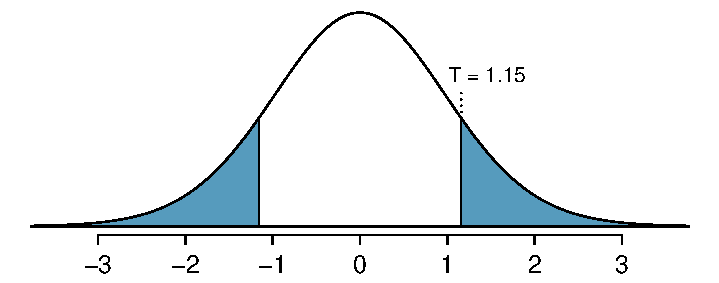
\includegraphics[width=0.8\textwidth]{ch_inference_for_means/figures/pValueOfTwoTailAreaOfExamVersionsWhereDFIs26/pValueOfTwoTailAreaOfExamVersionsWhereDFIs26}
\caption{The $t$ distribution with 26 degrees of freedom. The shaded right tail represents values with $T \geq 1.15$. Because it is a two-sided test, we also shade the corresponding lower tail.}
\label{pValueOfTwoTailAreaOfExamVersionsWhereDFIs26}
\end{figure}

\begin{exercise} \label{computeTwoTailAreaOfExamVersionsWhereDFIs26}
Identify the p-value, shown in Figure~\ref{pValueOfTwoTailAreaOfExamVersionsWhereDFIs26}. Use $df=26$.\footnote{We examine row $df=26$ in the $t$ table. Because this value is smaller than the value in the left column, the p-value is larger than 0.200 (two tails!). Because the p-value is so large, we do not reject the null hypothesis. That is, the data do not convincingly show that one exam version is more difficult than the other, and the teacher should not be convinced that she should add points to the Version B exam scores.}

\index{data!two exam comparison|)}

\end{exercise}

In Guided Practice~\ref{computeTwoTailAreaOfExamVersionsWhereDFIs26}, we could have used $df=45.97$. However, this value is not listed in the table. In such cases, we use the next lower degrees of freedom (unless the computer also provides the p-value). For example, we could have used $df=45$ but not $df=46$.
As before, we provide a summary of the steps to perform when carrying out such a test.


\begin{termBox}{\tBoxTitle[]{Hypothesis test for the difference of two means}
\begin{enumerate}
\setlength{\itemsep}{0mm}
\item State the name of the test being used: 2-sample t test.
\item Verify conditions.\vspace{-1.5mm}
\begin{itemize}
\setlength{\itemsep}{0mm}
\item 2 independent random samples OR 2 randomly allocated treatments
\item Both populations known to be normal OR $n_1 and n_2\ge 30$ OR graphs of both samples are approximately symmetric with no outliers, making the assumption that the populations are normal a reasonable one
\end{itemize}
\item Write the hypotheses in plain language, then set them up in mathematical notation.\vspace{-1.5mm}
\begin{itemize}
\setlength{\itemsep}{0mm}
\item H$_0: \mu_1 = \mu_2$ or  $\mu_1 - \mu_2 = 0$
\item H$_0: \mu_1 \ne \text{or} < \text{or} > \mu_2$
\end{itemize}
\item Identify the significance level $\alpha$.
\item Calculate the test statistic and $df$.
$$\text{t} = \frac{\text{point estimate} - \text{null value}}{\text{SE of estimate}}$$
Use a point estimate of $\bar{x}_1-\bar{x}_2$, compute $SE = \sqrt{\frac{s^2_1}{n_1}+\frac{s^2_2}{n_2}}$, and get the $df$ from a calculator.
\item Find the p-value and compare it to $\alpha$ to determine whether to reject or not reject $H_0$.
\item Write the conclusion in the context of the question.
\end{enumerate}}
\end{termBox}

\index{data!stem cells, heart function|(}

\begin{table}[h]
\centering
\begin{tabular}{l rrrrr}
\hline
\hspace{10mm}	& $n$	& $\bar{x}$	& $s$  	 \\
\hline
ESCs		& 9		& 3.50		& 5.17  	\\
control		& 9		& -4.33		& 2.76  	 \\
\hline
\end{tabular}
\caption{Summary statistics for the embryonic stem cell data set.}
\label{summaryStatsForSheepHeartDataWhoReceivedMiceESCs}
\end{table}

\begin{figure}
\centering
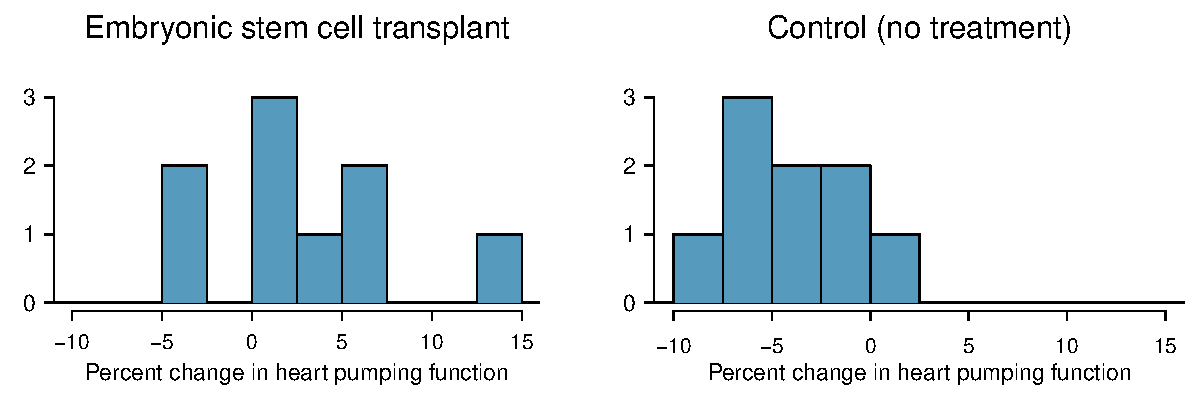
\includegraphics[width=\textwidth]{ch_inference_for_means/figures/stemCellTherapyForHearts/stemCellTherapyForHearts}
\caption{Histograms for both the embryonic stem cell group and the control group. Higher values are associated with greater improvement. We don't see any evidence of skew in these data; however, it is worth noting that skew would be difficult to detect with such a small sample.}
\label{stemCellTherapyForHearts}
\end{figure}

\textPE{\newpage}

\begin{example} {\label{exerciseToEvaluteWhetherESCsAreHelpfulInImprovingHeartFunctionInSheep}
Do embryonic stem cells (ESCs) help improve heart function following a heart attack? Table~\ref{summaryStatsForSheepHeartDataWhoReceivedMiceESCs} contains summary statistics for an experiment to test ESCs in sheep that had a heart attack. Each of these sheep was randomly assigned to the ESC or control group, and the change in their hearts' pumping capacity was measured. A positive value generally corresponds to increased pumping capacity, which suggests a stronger recovery. The sample data is graphed in Figure~\ref{stemCellTherapyForHearts}. Use the given information and an appropriate an appopriate statistical test to answer the research question.
}
We will carry out a 2-sample t test. The first condition is met because it is stated that there were two randomly allocated treatments. For the second condition, we must look at a graphs of the data. The data are very limited, so we can only check for obvious outliers in the raw data in Figure~\ref{stemCellTherapyForHearts}. Since the distributions are (very) roughly symmetric, we will assume the populations are approximately normal.
\begin{itemize}
\setlength{\itemsep}{0mm}
\item[$H_0$:] $\mu_{esc} - \mu_{control} = 0$. The stem cells do not improve heart pumping function.
\item[$H_A$:] $\mu_{esc} - \mu_{control} > 0$. The stem cells do improve heart pumping function.
\end{itemize}
Let $\alpha=0.05$. Now we compute the sample difference, the standard error for that point estimate, and the test statistic:
\begin{align*}
& \bar{x}_{esc} - \bar{x}_{control} = 7.83
&& SE = \sqrt{\frac{5.17^2}{9} + \frac{2.76^2}{9}} = 1.95
&&T = \frac{7.83 - 0}{1.95} = 4.01
\end{align*}
Using a calculator, $df=12.2$ and p-value = $8.4\text{x}10^{-4}$. The p-value is much less than 0.05, so we reject the null hypothesis. The data provide convincing evidence that embryonic stem cells improve the heart's pumping function in sheep that have suffered a heart attack.
\end{example}

\textPE{\pagebreak}


\subsection{Confidence intervals for $\mu_1-\mu_2$}

The results from the previous section provided evidence that ESCs actually help improve the pumping function of the heart. But how large is this improvement? To answer this question, we can use a confidence interval.

Confidence intervals take the form
\begin{align*}
\text{point estimate} \ \pm \text{critical value }\times SE
\end{align*}
Using the point estimate and the SE calculated in the previous section, we get the general form of a confidence interval for a difference in means, $\mu_1-\mu_2$.
\begin{align*}
(\bar{x}_1-\bar{x}_2) \ \pm \ t^\star\sqrt{\frac{s_1^2}{n_1} + \frac{s_2^2}{n_2}}
\end{align*}

\begin{exercise}
In Example~\ref{exerciseToEvaluteWhetherESCsAreHelpfulInImprovingHeartFunctionInSheep}, you found that the point estimate, $\bar{x}_{esc} - \bar{x}_{control} = 7.83$, has a standard error of 1.95. Using $df=8$, create a 99\% confidence interval for the improvement due to ESCs.\footnote{We know the point estimate, 7.83, and the standard error, 1.95. We also verified the conditions for using the $t$ distribution in Example~\ref{exerciseToEvaluteWhetherESCsAreHelpfulInImprovingHeartFunctionInSheep}. Thus, we only need identify $t^{\star}_8$ to create a 99\% confidence interval: $t^{\star}_{8} = 3.36$. The 99\% confidence interval for the improvement from ESCs is given by
\begin{align*}
\text{point estimate}\ &\pm\ t^{\star}SE \\
7.83\ &\pm\ 3.36\times 1.95 \quad  df=8\\
(1.33 &\text{ , } 14.43)
\end{align*}
That is, we are 99\% confident that the true improvement in heart pumping function is somewhere between 1.33\% and 14.43\%.}

\index{data!stem cells, heart function|)}

\end{exercise}

%\begin{exercise}
%What does 95\% confidence mean?\footnote{If we were to collected many such samples and create 95\% confidence intervals for each, then about 95\% of these intervals would contain the population difference, $\mu_w - \mu_m$.}
%\end{exercise}

\begin{termBox}{\tBoxTitle[]{Constructing a confidence interval for the difference of two means}
\begin{enumerate}
\setlength{\itemsep}{0mm}
\item State the name of the CI being used: 2-sample t interval.
\item Verify conditions.\vspace{-1.5mm}
\begin{itemize}
\item 2 independent random samples OR 2 randomly allocated treatments
\item Both populations are known to be normal OR $n_1 \text{ and } n_2\ge 30$ OR graphs of both samples are approximately symmetric with no outliers, making the assumption that the populations are normal a reasonable one
\end{itemize}
\item Plug in the numbers and write the interval in the form
$$\text{point estimate } \pm \text{ critical value}\times \text{SE of estimate}$$
Compute the point estimate as $\bar{x}_1-\bar{x}_2$, get the $df$ from a calculator, find the critical value $t^\star$ using the t table at row = $df$, and compute $SE = \sqrt{\frac{s^2_1}{n_1}+\frac{s^2_2}{n_2}}$.
\item Evaluate the CI and write in the form ( $\_$ , $\_$ ).
\item Interpret the interval:  ``We are [XX]\% confident that the true difference in the mean of [...] is between [...] and [...]."
\item State your conclusion to the original question.
\end{enumerate}}
\end{termBox}


An instructor decided to run two slight variations of the same exam. Prior to passing out the exams, she shuffled the exams together to ensure each student received a random version. Summary statistics for how students performed on these two exams are shown in Table~\ref{summaryStatsForTwoVersionsOfExams2nd}. Anticipating complaints from students who took Version~B, she would like to evaluate whether the difference observed in the groups is so large that it provides convincing evidence that Version~B was more difficult (on average) than Version~A.

\begin{table}[hht]
\centering
\begin{tabular}{l rrrrr}
\hline
Version\hspace{2mm}	& $n$	& $\bar{x}$	& $s$	& min	& max  \\
\hline
A		& 30		& 79.4		& 14 	& 45		& 100 \\
B		& 27		& 74.1		& 20		& 32		& 100 \\
\hline
\end{tabular}
\caption{Summary statistics of scores for each exam version.}
\label{summaryStatsForTwoVersionsOfExams2nd}
\end{table}

\begin{example}{Construct a 90\% confidence interval for the difference in average scores. At this confidence level, is there evidence that test was more difficult than the other?}We have two randomly allocated treatments (tests) and the scores for both groups do not show excessive skew, so we can assume that the population distributions are approximately normal. The point estimate is $\bar{x}_A - \bar{x}_B = 5.3$. The standard error of the estimate can be calculated~as
\begin{eqnarray*}
SE = \sqrt{\frac{14^2}{30} + \frac{20^2}{27}} = 4.62
\end{eqnarray*}
A calculator gives the degrees of freedom as 45.97.
The confidence interval is given by $5.3\ \pm \ 1.684(4.62)\to (-2.5, 13.1)$. Because the interval contains both positive and negative values the data do not convincingly show that one exam version is more difficult than the other, and the teacher should not be convinced that she should add points to the Version B exam scores.
\index{data!two exam comparison|)}
\end{example}

\textPE{\newpage}


\subsection{Calculator: The 2-sample t test and CI\vspace{-3mm}}

\begin{termBox}{\tBoxTitle{TI calculator: Carrying out the 2-sample t test}
Use \textbf{STAT, TESTS, 2-SampTTest}.\vspace{-1.5mm}
\begin{enumerate}
\setlength{\itemsep}{0mm}
\item Choose STAT.
\item Right arrow to TESTS.
\item Choose 4: 2-SampTTest
\item Choose Data if you have all the data or Stats if you have the means and standard deviations.\vspace{-1.5mm}
\begin{itemize}
\setlength{\itemsep}{0mm}
\item If you choose Data, let List1 be L1 or the list that contains sample 1 and let List2 be L2 or the list that contains sample 2 (don't forget to enter the data!). Let Freq1 and Freq2 be 1.
\item If you choose Stats, enter the mean, SD, and sample size for sample 1 and for sample 2
\end{itemize}
\item Choose $\ne$, $<$, or $>$ to correspond to H$_A$.
\item Let Pooled be NO.
\item Choose Calculate and hit ENTER, which returns: \\
\begin{tabular}{ll ll}
t
	&\quad t statistic
	&\quad Sx1
	&\quad SD of sample 1 \\
p
	&\quad p-value
	&\quad Sx2
	&\quad SD of sample 2 \\
df
	&\quad degrees of freedom
	&\quad n1
	&\quad size of sample 1 \\
$\bar{x}_1$
	&\quad mean of sample 1
	&\quad n2
	&\quad size of sample 2 \\
$\bar{x}_2$
	&\quad mean of sample 2
\end{tabular}
\end{enumerate}
}
\end{termBox}

\begin{termBox}{\tBoxTitle{TI calculator: Calculating the 2-sample t Confidence Interval}Use \textbf{STAT, TESTS, 2-SampTInt}.\vspace{-1.5mm}
\begin{enumerate}
\setlength{\itemsep}{0mm}
\item Choose STAT.
\item Right arrow to TESTS.
\item Down arrow and choose 0: 2-SampTTInt.
\item Choose Data if you have all the data or Stats if you have the means and standard deviations.\vspace{-1.5mm}
\begin{itemize}
\setlength{\itemsep}{0mm}
\item If you choose Data, let List1 be L1 or the list that contains sample 1 and let List2 be L2 or the list that contains sample 2 (don't forget to enter the data!). Let Freq1 and Freq2 be 1.
\item If you choose Stats, enter the mean, SD, and sample size for sample 1 and for sample 2.
\end{itemize}
\item Let C-Level be the desired confidence level and let Pooled be No.
\item Choose Calculate and hit ENTER, which returns: \\
\begin{tabular}{ll ll}
( $\_$ , $\_$ )
	&\quad the confidence interval
	&\quad Sx1
	&\quad SD of sample 1 \\
df
	&\quad degrees of freedom
	&\quad Sx2
	&\quad SD of sample 2 \\
$\bar{x}_1$
	&\quad mean of sample 1
	&\quad n1
	&\quad size of sample 1 \\
$\bar{x}_2$
	&\quad mean of sample 2
	&\quad n2
	&\quad size of sample 2
\end{tabular}
\end{enumerate}
}
\end{termBox}

\begin{exercise}Use the data from the ESC experiment shown in Table~\ref{summaryStatsForSheepHeartDataWhoReceivedMiceESCsForCalcSubsection} and a calculator to construct a 90\% confidence interval.\footnote{The interval is $(4.3543, 11.307)$ with $df=12.2$.}
\end{exercise}

\begin{table}
\centering
\begin{tabular}{l rrrrr}
\hline
\hspace{10mm}	& $n$	& $\bar{x}$	& $s$  	 \\
\hline
ESCs		& 9		& 3.50		& 5.17  	\\
control		& 9		& -4.33		& 2.76  	 \\
\hline
\end{tabular}
\caption{Summary statistics for the embryonic stem cell data set.}
\label{summaryStatsForSheepHeartDataWhoReceivedMiceESCsForCalcSubsection}
\end{table}

\begin{exercise}Use the data from the ESC example and a calculator to find an appropriate statistic, degrees of freedom, and p-value for a two-sided hypothesis test.\footnote{$t=4.008$, $df=12.2$, and p-value$=0.00168$.}
\end{exercise}



%__________________
\section[Comparing many means with ANOVA (special topic)]{Comparing many means with ANOVA\\(special topic)}
\label{anovaAndRegrWithCategoricalVariables}

\index{analysis of variance (ANOVA)|(}

Sometimes we want to compare means across many groups. We might initially think to do pairwise comparisons; for example, if there were three groups, we might be tempted to compare the first mean with the second, then with the third, and then finally compare the second and third means for a total of three comparisons. However, this strategy can be treacherous. If we have many groups and do many comparisons, it is likely that we will eventually find a difference just by chance, even if there is no difference in the populations.

In this section, we will learn a new method called \term{analysis of variance (ANOVA)} and a new test statistic called $F$. ANOVA uses a single hypothesis test to check whether the means across many groups are equal:
\begin{itemize}
\setlength{\itemsep}{0mm}
\item[$H_0$:] The mean outcome is the same across all groups. In statistical notation, $\mu_1 = \mu_2 = \cdots = \mu_k$ where $\mu_i$ represents the mean of the outcome for observations in category $i$.
\item[$H_A$:] At least one mean is different.
\end{itemize}
Generally we must check three conditions on the data before performing ANOVA:
\begin{itemize}
\setlength{\itemsep}{0mm}
\item the observations are independent within and across groups,
\item the data within each group are nearly normal, and
\item the variability across the groups is about equal.
\end{itemize}
When these three conditions are met, we may perform an ANOVA to determine whether the data provide strong evidence against the null hypothesis that all the $\mu_i$ are equal.

\textPE{\newpage}

\begin{example}{College departments commonly run multiple lectures of the same introductory course each semester because of high demand. Consider a statistics department that runs three lectures of an introductory statistics course. We might like to determine whether there are statistically significant differences in first exam scores in these three classes ($A$, $B$, and $C$). Describe appropriate hypotheses to determine whether there are any differences between the three classes.} \label{firstExampleForThreeStatisticsClassesAndANOVA}
The hypotheses may be written in the following form:
\begin{itemize}
\setlength{\itemsep}{0mm}
\item[$H_0$:] The average score is identical in all lectures. Any observed difference is due to chance. Notationally, we write $\mu_A=\mu_B=\mu_C$.
\item[$H_A$:] The average score varies by class. We would reject the null hypothesis in favor of the alternative hypothesis if there were larger differences among the class averages than what we might expect from chance alone.
\end{itemize}
\end{example}

Strong evidence favoring the alternative hypothesis in ANOVA is described by unusually large differences among the group means. We will soon learn that assessing the variability of the group means relative to the variability among individual observations within each group is key to ANOVA's success.

\begin{example}{Examine Figure~\ref{toyANOVA}. Compare groups I, II, and III. Can you visually determine if the differences in the group centers is due to chance or not? Now compare groups IV, V, and VI. Do these differences appear to be due to chance?}

\begin{figure}[h]
\centering
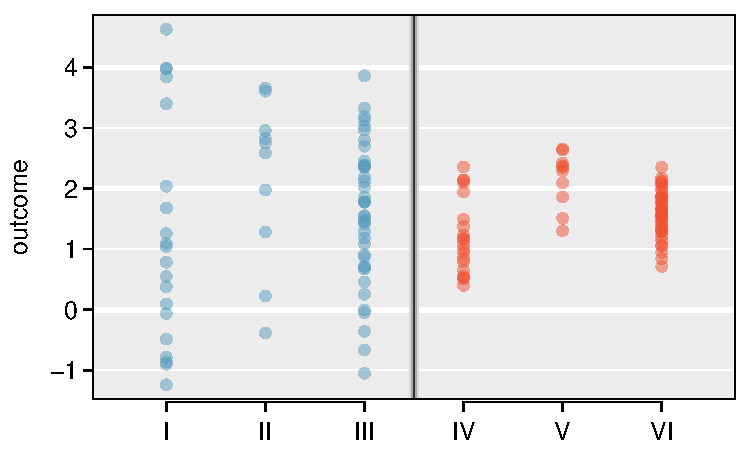
\includegraphics[width=0.65\textwidth]{ch_inference_for_means/figures/toyANOVA/toyANOVA}
\caption{Side-by-side dot plot for the outcomes for six groups.\vspaceB{-3.5mm}}
\label{toyANOVA}
\end{figure}

Any real difference in the means of groups I, II, and III is difficult to discern, because the data within each group are very volatile relative to any differences in the average outcome. On the other hand, it appears there are differences in the centers of groups IV, V, and VI. For instance, group V appears to have a higher mean than that of the other two groups. Investigating groups IV, V, and VI, we see the differences in the groups' centers are noticeable because those differences are large \emph{relative to the variability in the individual observations within each group}.
\end{example}

\textPE{\newpage}


\subsection{Is batting performance related to player position in MLB?}

\index{data!MLB batting|(}

We would like to discern whether there are real differences between the batting performance of baseball players according to their position: outfielder (\resp{OF}), infielder (\resp{IF}), designated hitter (\resp{DH}), and catcher (\resp{C}). We will use a data set called \data{bat10}, which includes batting records of 327 Major League Baseball (MLB) players from the 2010 season. Six of the 327 cases represented in \data{bat10} are shown in Table~\ref{mlbBat10DataMatrix}, and descriptions for each variable are provided in Table~\ref{mlbBat10Variables}. The measure we will use for the player batting performance (the outcome variable) is on-base percentage (\var{OBP}). The on-base percentage roughly represents the fraction of the time a player successfully gets on base or hits a home run.

\begin{table}[h]
\centering
\begin{tabular}{rlllrrrrrr}
  \hline
 & name & team & position & AB & H & HR &RBI & AVG & OBP \\
  \hline
1 & I Suzuki & SEA & OF & 680 & 214 & 6 & 43 & 0.315 & 0.359 \\
  2 & D Jeter & NYY & IF & 663 & 179 & 10 & 67 & 0.270 & 0.340 \\
  3 & M Young & TEX & IF & 656 & 186 & 21 & 91 & 0.284 & 0.330 \\
  $\vdots$ & $\vdots$ & $\vdots$ & $\vdots$ & $\vdots$ & $\vdots$ & $\vdots$ & $\vdots$ \\
  325 & B Molina & SF & C & 202 & 52 & 3 & 17 & 0.257 & 0.312 \\
  326 & J Thole & NYM & C & 202 & 56 & 3 & 17 & 0.277 & 0.357 \\
  327 & C Heisey & CIN & OF & 201 & 51 & 8 & 21 & 0.254 & 0.324 \\
   \hline
\end{tabular}
\caption{Six cases from the \data{bat10} data matrix.\vspaceB{-3mm}}
\label{mlbBat10DataMatrix}
\end{table}

\begin{table}[h]
\centering\small
\begin{tabular}{lp{8.5cm}}
\hline
{\bf variable} & {\bf description} \\
\hline
\var{name} & Player name \\
\var{team} & The abbreviated name of the player's team \\
\var{position} & The player's primary field position (\resp{OF}, \resp{IF}, \resp{DH}, \resp{C}) \\
\var{AB} & Number of opportunities at bat \\
\var{H} & Number of hits \\
\var{HR} & Number of home runs \\
\var{RBI} & Number of runs batted in \\
\var{AVG} & Batting average, which is equal to $\resp{H}/\resp{AB}$ \\
\var{OBP} & On-base percentage, which is roughly equal to the fraction of times a player gets on base or hits a home run \\
\hline
\end{tabular}
\caption{Variables and their descriptions for the \data{bat10} data set.}
\label{mlbBat10Variables}
\end{table}

\begin{exercise} \label{nullHypForOBPAgainstPosition}
The null hypothesis under consideration is the following: $\mu_{\resp{OF}} = \mu_{\resp{IF}} = \mu_{\resp{DH}} = \mu_{\resp{C}}$.
Write the null and corresponding alternative hypotheses in plain language.\footnote{$H_0$: The average on-base percentage is equal across the four positions.\\\noindent $H_A$: The average on-base percentage varies across some (or all) groups.}
\end{exercise}

\textB{\pagebreak}

\begin{example}{The player positions have been divided into four groups: outfield (\resp{OF}), infield (\resp{IF}), designated hitter (\resp{DH}), and catcher (\resp{C}). What would be an appropriate point estimate of the on-base percentage by outfielders, $\mu_{\resp{OF}}$?}
A good estimate of the on-base percentage by outfielders would be the sample average of \var{AVG} for just those players whose position is outfield: $\bar{x}_{OF} = 0.334$.
\end{example}

Table~\ref{mlbHRPerABSummaryTable} provides summary statistics for each group. A side-by-side box plot for the on-base percentage is shown in Figure~\ref{mlbANOVABoxPlot}. Notice that the variability appears to be approximately constant across groups; nearly constant variance across groups is an important assumption that must be satisfied before we consider the ANOVA approach.

\begin{table}[ht]
\centering\small
\begin{tabular}{lrrrr}
\hline
	& \resp{OF} & \resp{IF} & \resp{DH} & \resp{C} \\
\hline
Sample size ($n_i$)	& 120 & 154 & 14 & 39 \\
Sample mean ($\bar{x}_i$)	& 0.334 & 0.332 & 0.348 & 0.323 \\
Sample SD ($s_i$)	& 0.029 & 0.037 & 0.036 & 0.045 \\
\hline
\end{tabular}
\caption{Summary statistics of on-base percentage, split by player position.}
\label{mlbHRPerABSummaryTable}
\end{table}

\begin{figure}
\centering
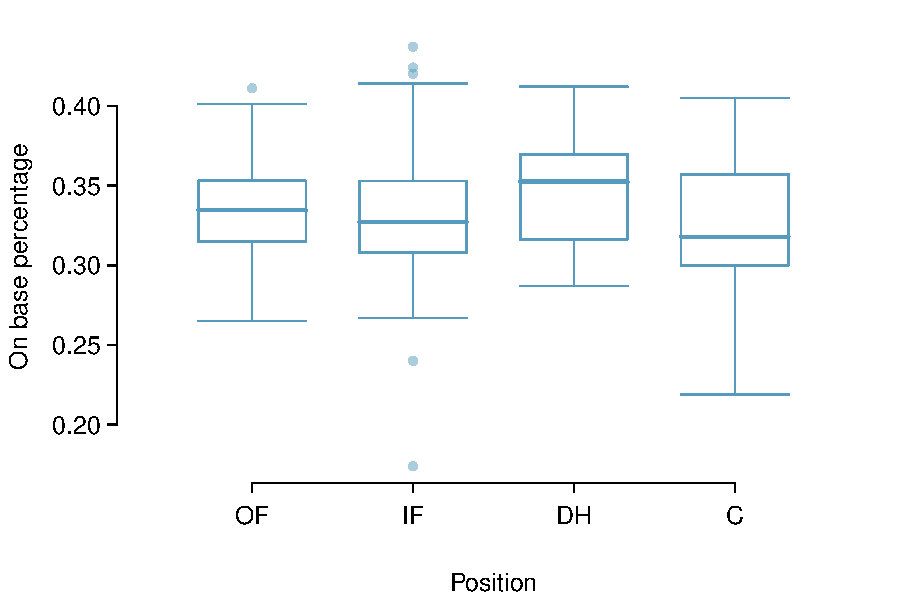
\includegraphics[width=0.85\textwidth]{ch_inference_for_means/figures/mlbANOVA/mlbANOVABoxPlot}
\caption{Side-by-side box plot of the on-base percentage for 327 players across four groups. There is one prominent outlier visible in the infield group, but with 154 observations in the infield group, this outlier is not a concern.}
\label{mlbANOVABoxPlot}
\end{figure}

\textPE{\newpage}

\begin{example}{The largest difference between the sample means is between the designated hitter and the catcher positions. Consider again the original hypotheses:
\begin{itemize}
\setlength{\itemsep}{0mm}
\item[$H_0$:] $\mu_{\resp{OF}} = \mu_{\resp{IF}} = \mu_{\resp{DH}} = \mu_{\resp{C}}$
\item[$H_A$:] The average on-base percentage ($\mu_i$) varies across some (or all) groups.
\end{itemize}
Why might it be inappropriate to run the test by simply estimating whether the difference of $\mu_{\var{DH}}$ and $\mu_{\resp{C}}$ is statistically significant at a 0.05 significance level?}
\label{multipleComparisonExampleThatIncludesDiscussionOfClassrooms}
The primary issue here is that we are inspecting the data before picking the groups that will be compared. It is inappropriate to examine all data by eye (informal testing) and only afterwards decide which parts to formally test. This is called \term{data snooping} or \term{data fishing}. Naturally we would pick the groups with the large differences for the formal test, leading to an inflation in the Type 1 Error rate. To understand this better, let's consider a slightly different problem.

Suppose we are to measure the aptitude for students in 20 classes in a large elementary school at the beginning of the year. In this school, all students are randomly assigned to classrooms, so any differences we observe between the classes at the start of the year are completely due to chance. However, with so many groups, we will probably observe a few groups that look rather different from each other. If we select only these classes that look so different, we will probably make the wrong conclusion that the assignment wasn't random. While we might only formally test differences for a few pairs of classes, we informally evaluated the other classes by eye before choosing the most extreme cases for a comparison.
\end{example}

For additional information on the ideas expressed in Example~\ref{multipleComparisonExampleThatIncludesDiscussionOfClassrooms}, we recommend reading about the \term{prosecutor's fallacy}.\footnote{See, for example, \href{http://www.stat.columbia.edu/~cook/movabletype/archives/2007/05/the_prosecutors.html}{www.stat.columbia.edu/$\sim$cook/movabletype/archives/2007/05/the\_prosecutors.html}.}

In the next section we will learn how to use the $F$ statistic and ANOVA to test whether observed differences in means could have happened just by chance even if there was no difference in the respective population means.


\subsection{Analysis of variance (ANOVA) and the F test}

The method of analysis of variance in this context focuses on answering one question: is the variability in the sample means so large that it seems unlikely to be from chance alone? This question is different from earlier testing procedures since we will \emph{simultaneously} consider many groups, and evaluate whether their sample means differ more than we would expect from natural variation. We call this variability the \term{mean square between groups ($MSG$)}, and it has an associated degrees of freedom, $df_{G}=k-1$ when there are $k$ groups. The $MSG$ can be thought of as a scaled variance formula for means. If the null hypothesis is true, any variation in the sample means is due to chance and shouldn't be too large. Details of $MSG$ calculations are provided in the footnote,\footnote{Let $\bar{x}$ represent the mean of outcomes across all groups. Then the mean square between groups is computed as
\begin{align*}
MSG = \frac{1}{df_{G}}SSG = \frac{1}{k-1}\sum_{i=1}^{k} n_{i}\left(\bar{x}_{i} - \bar{x}\right)^2
\end{align*}
where $SSG$ is called the \term{sum of squares between groups} and $n_{i}$ is the sample size of group $i$.} however, we typically use software for these computations.

The mean square between the groups is, on its own, quite useless in a hypothesis test. We need a benchmark value for how much variability should be expected among the sample means if the null hypothesis is true. To this end, we compute a pooled variance estimate, often abbreviated as the \term{mean square error ($MSE$)}, which has an associated degrees of freedom value $df_E=n-k$. It is helpful to think of $MSE$ as a measure of the variability within the groups. Details of the computations of the $MSE$ are provided in the footnote\footnote{Let $\bar{x}$ represent the mean of outcomes across all groups. Then the \term{sum of squares total ($SST$)} is computed as
\begin{align*}
SST = \sum_{i=1}^{n} \left(x_{i} - \bar{x}\right)^2
\end{align*}
where the sum is over all observations in the data set. Then we compute the \term{sum of squared errors ($SSE$)} in one of two equivalent ways:
\begin{align*}
SSE &= SST - SSG \\
	&= (n_1-1)s_1^2 + (n_2-1)s_2^2 + \cdots + (n_k-1)s_k^2
\end{align*}
where $s_i^2$ is the sample variance (square of the standard deviation) of the residuals in group $i$. Then the $MSE$ is the standardized form of $SSE$: $MSE = \frac{1}{df_{E}}SSE$.} for interested readers.

When the null hypothesis is true, any differences among the sample means are only due to chance, and the $MSG$ and $MSE$ should be about equal. As a test statistic for ANOVA, we examine the fraction of $MSG$ and $MSE$:
\begin{align} \label{formulaForTheFStatistic}
F = \frac{MSG}{MSE}
\end{align}
The $MSG$ represents a measure of the between-group variability, and $MSE$ measures the variability within each of the groups.

\begin{exercise}
For the baseball data, $MSG = 0.00252$ and $MSE=0.00127$. Identify the degrees of freedom associated with MSG and MSE and verify the $F$ statistic is approximately 1.994.\footnote{There are $k=4$ groups, so $df_{G} = k-1 = 3$. There are $n = n_1 + n_2 + n_3 + n_4 = 327$ total observations, so $df_{E} = n - k = 323$. Then the $F$ statistic is computed as the ratio of $MSG$ and $MSE$: $F = \frac{MSG}{MSE} = \frac{0.00252}{0.00127} = 1.984 \approx 1.994$. ($F=1.994$ was computed by using values for $MSG$ and $MSE$ that were not rounded.)}
\end{exercise}

We can use the $F$ statistic to evaluate the hypotheses in what is called an \term{F test}. A p-value can be computed from the $F$ statistic using an $F$ distribution, which has two associated parameters: $df_{1}$ and $df_{2}$. For the $F$ statistic in ANOVA, $df_{1} = df_{G}$ and $df_{2}= df_{E}$. An $F$ distribution with 3 and 323 degrees of freedom, corresponding to the $F$ statistic for the baseball hypothesis test, is shown in Figure~\ref{fDist3And323}.

\begin{figure}[ht]
\centering
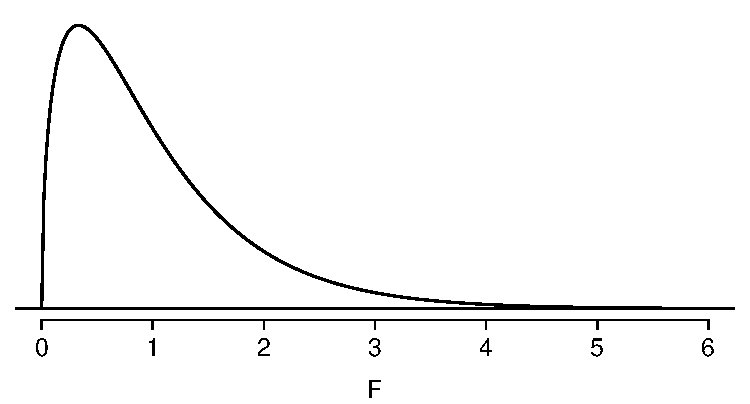
\includegraphics[width=0.7\textwidth]{ch_inference_for_means/figures/fDist3And323/fDist3And323}
\caption{An $F$ distribution with $df_1=3$ and $df_2=323$.}
\label{fDist3And323}
\end{figure}

The larger the observed variability in the sample means ($MSG$) relative to the within-group observations ($MSE$), the larger $F$ will be and the stronger the evidence against the null hypothesis. Because larger values of $F$ represent stronger evidence against the null hypothesis, we use the upper tail of the distribution to compute a p-value.

\begin{termBox}{\tBoxTitle{The $F$ statistic and the $F$ test}
Analysis of variance (ANOVA) is used to test whether the mean outcome differs across 2 or more groups. ANOVA uses a test statistic $F$, which represents a standardized ratio of variability in the sample means relative to the variability within the groups. If $H_0$ is true and the model assumptions are satisfied, the statistic $F$ follows an $F$ distribution with parameters $df_{1}=k-1$ and $df_{2}=n-k$. The upper tail of the $F$ distribution is used to represent the p-value.}
\end{termBox}

\begin{exercise}\label{describePValueAreaForFDistributionInMLBOBPExample}
The test statistic for the baseball example is $F=1.994$. Shade the area corresponding to the p-value in Figure~\ref{fDist3And323}. \footnote{\ \vspace{-4mm}\\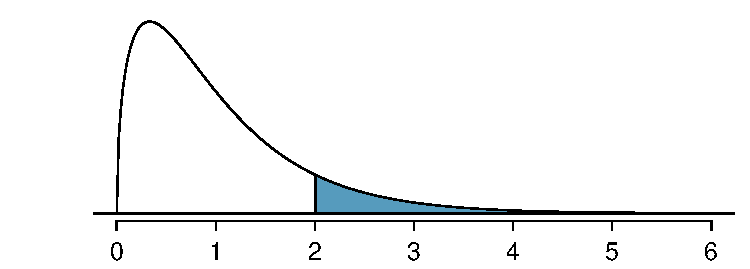
\includegraphics[height=20mm]{ch_inference_for_means/figures/fDist3And323/fDist3And323Shaded}}
\end{exercise}

\begin{example}{The p-value corresponding to the shaded area in the solution of Guided Practice~\ref{describePValueAreaForFDistributionInMLBOBPExample} is equal to about 0.115. Does this provide strong evidence against the null hypothesis?}
The p-value is larger than 0.05, indicating the evidence is not strong enough to reject the null hypothesis at a significance level of 0.05. That is, the data do not provide strong evidence that the average on-base percentage varies by player's primary field position.
\end{example}


\subsection{Reading an ANOVA table from software}

The calculations required to perform an ANOVA by hand are tedious and prone to human error. For these reasons, it is common to use statistical software to calculate the $F$ statistic and p-value.

An ANOVA can be summarized in a table very similar to that of a regression summary, which we will see in Chapter~\ref{linRegrForTwoVar}. Table~\ref{anovaSummaryTableForOBPAgainstPosition} shows an ANOVA summary to test whether the mean of on-base percentage varies by player positions in the MLB. Many of these values should look familiar; in particular, the $F$ test statistic and p-value can be retrieved from the last columns.

\begin{table}[ht]
\centering
\begin{tabular}{lrrrrr}
  \hline
 & Df & Sum Sq & Mean Sq & F value & Pr($>$F) \\
  \hline
position & 3 & 0.0076 & 0.0025 & 1.9943 & 0.1147 \\
  Residuals & 323 & 0.4080 & 0.0013 &  &  \\    \hline
\multicolumn{6}{r}{$s_{pooled} = 0.036$ on $df=323$}
\end{tabular}
\caption{ANOVA summary for testing whether the average on-base percentage differs across player positions.}
\label{anovaSummaryTableForOBPAgainstPosition}
\end{table}


\subsection{Graphical diagnostics for an ANOVA analysis}

There are three conditions we must check for an ANOVA analysis: all observations must be independent, the data in each group must be nearly normal, and the variance within each group must be approximately equal.

\begin{description}
\item[Independence.] If the data are a simple random sample from less than 10\% of the population, this condition is satisfied. For processes and experiments, carefully consider whether the data may be independent (e.g. no pairing). For example, in the MLB data, the data were not sampled. However, there are not obvious reasons why independence would not hold for most or all observations.
\item[Approximately normal.] As with one- and two-sample testing for means, the normality assumption is especially important when the sample size is quite small. The normal probability plots for each group of the MLB data are shown in Figure~\ref{mlbANOVADiagNormalityGroups}; there is some deviation from normality for infielders, but this isn't a substantial concern since there are about 150 observations in that group and the outliers are not extreme. Sometimes in ANOVA there are so many groups or so few observations per group that checking normality for each group isn't reasonable. See the footnote\footnote{First calculate the \termsub{residuals}{residual} of the baseball data, which are calculated by taking the observed values and subtracting the corresponding group means. For example, an outfielder with OBP of 0.435 would have a residual of $0.405 - \bar{x}_{OF} = 0.071$. Then to check the normality condition, create a normal probability plot using all the residuals simultaneously.} for guidance on how to handle such instances.

\begin{figure}[hhh]
\centering
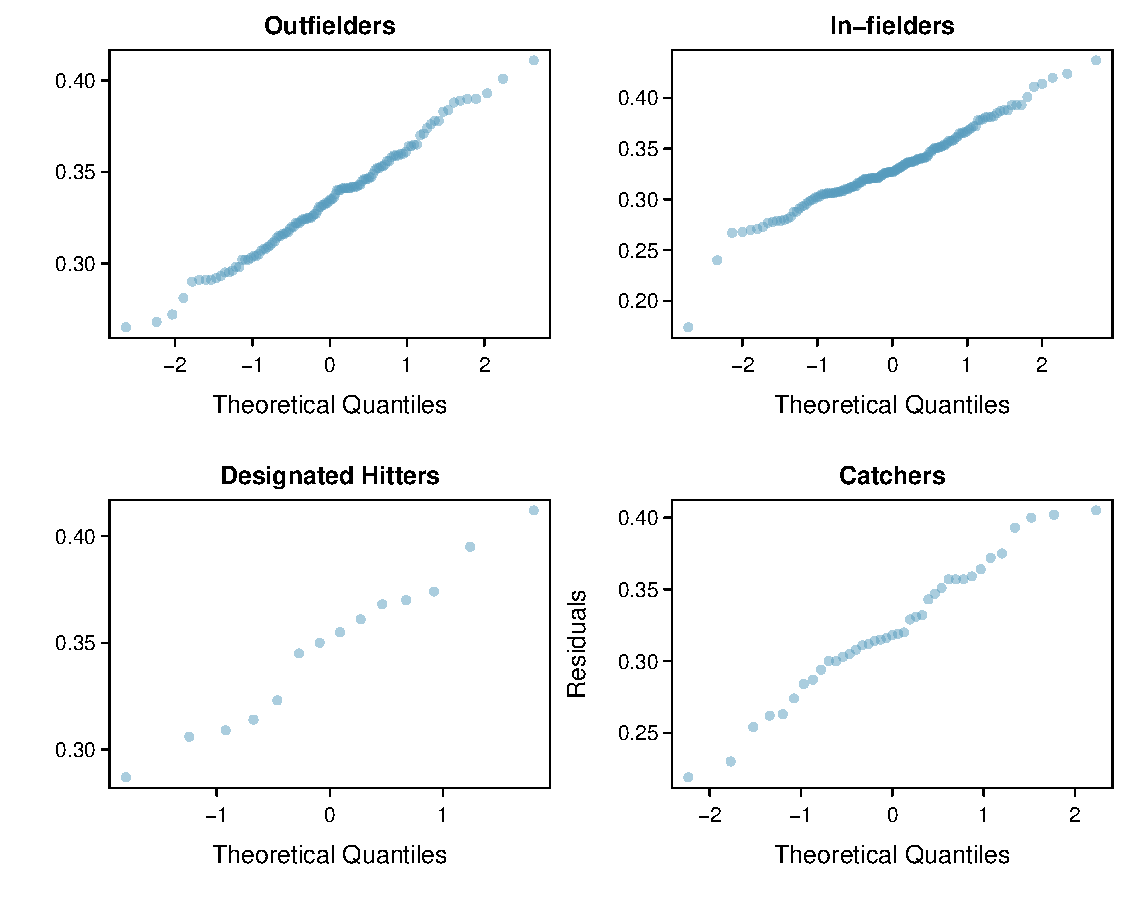
\includegraphics[width=\textwidth]{ch_inference_for_means/figures/mlbANOVA/mlbANOVADiagNormalityGroups}
\caption{Normal probability plot of OBP for each field position.}
\label{mlbANOVADiagNormalityGroups}
\end{figure}

\item[Constant variance.] The last assumption is that the variance in the groups is about equal from one group to the next. This assumption can be checked by examining a side-by-side box plot of the outcomes across the groups, as in Figure~\vref{mlbANOVABoxPlot}. In this case, the variability is similar in the four groups but not identical. We see in Table~\vref{mlbHRPerABSummaryTable} that the standard deviation varies a bit from one group to the next. Whether these differences are from natural variation is unclear, so we should report this uncertainty with the final results.

\index{data!MLB batting|)}

\end{description}

\begin{caution}
{Diagnostics for an ANOVA analysis}
{Independence is always important to an ANOVA analysis. The normality condition is very important when the sample sizes for each group are relatively small. The constant variance condition is especially important when the sample sizes differ between groups.}
\end{caution}


\subsection{Multiple comparisons and controlling Type 1 Error rate}
\label{multipleComparisonsAndControllingTheType1ErrorRate}

\index{significance level!multiple comparisons|(}

When we reject the null hypothesis in an ANOVA analysis, we might wonder, which of these groups have different means? To answer this question, we compare the means of each possible pair of groups. For instance, if there are three groups and there is strong evidence that there are some differences in the group means, there are three comparisons to make: group 1 to group 2, group 1 to group 3, and group 2 to group 3. These comparisons can be accomplished using a two-sample $t$ test, but we use a modified significance level and a pooled estimate of the standard deviation across groups. Usually this pooled standard deviation can be found in the ANOVA table, e.g. along the bottom of Table~\ref{anovaSummaryTableForOBPAgainstPosition}.

\textB{\newpage}

\begin{example}{Example~\vref{firstExampleForThreeStatisticsClassesAndANOVA} discussed three statistics lectures, all taught during the same semester. Table~\ref{summaryStatisticsForClassTestData} shows summary statistics for these three courses, and a side-by-side box plot of the data is shown in Figure~\ref{classDataSBSBoxPlot}. We would like to conduct an ANOVA for these data. Do you see any deviations from the three conditions for ANOVA?}
In this case (like many others) it is difficult to check independence in a rigorous way. Instead, the best we can do is use common sense to consider reasons the assumption of independence may not hold. For instance, the independence assumption may not be reasonable if there is a star teaching assistant that only half of the students may access; such a scenario would divide a class into two subgroups. No such situations were evident for these particular data, and we believe that independence is acceptable.

The distributions in the side-by-side box plot appear to be roughly symmetric and show no noticeable outliers.

The box plots show approximately equal variability, which can be verified in Table~\ref{summaryStatisticsForClassTestData}, supporting the constant variance assumption.
\end{example}

\begin{table}
\centering
\begin{tabular}{lrrr}
  \hline
Class $i$	& A	& B	& C \\
  \hline
$n_i$		& 58	& 55	& 51 \\
$\bar{x}_i$	& 75.1	& 72.0	& 78.9 \\
$s_i$		& 13.9	& 13.8	& 13.1 \\
\hline
\end{tabular}
\caption{Summary statistics for the first midterm scores in three different lectures of the same course.}
\label{summaryStatisticsForClassTestData}
\end{table}

\begin{figure}
\centering
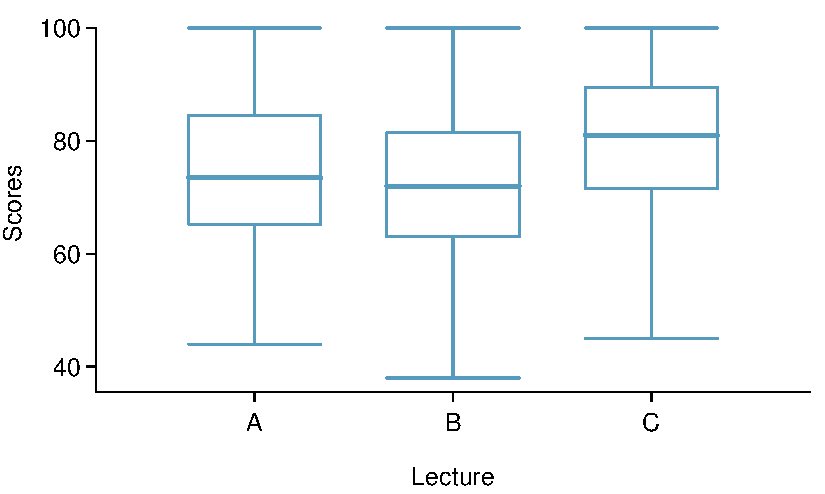
\includegraphics[width=0.8\textwidth]{ch_inference_for_means/figures/classData/classDataSBSBoxPlot}
\caption{Side-by-side box plot for the first midterm scores in three different  lectures of the same course.}
\label{classDataSBSBoxPlot}
\end{figure}

\begin{exercise} \label{exerExaminingAnovaSummaryTableForMidtermData}
An ANOVA was conducted for the midterm data, and summary results are shown in Table~\ref{anovaSummaryTableForMidtermData}. What should we conclude?\footnote{The p-value of the test is 0.0330, less than the default significance level of 0.05. Therefore, we reject the null hypothesis and conclude that the difference in the average midterm scores are not due to chance.}
\end{exercise}

\begin{table}
\centering
\begin{tabular}{lrrrrr}
  \hline
 & Df & Sum Sq & Mean Sq & F value & Pr($>$F) \\
  \hline
lecture & 2 & 1290.11 & 645.06 & 3.48 & 0.0330 \\
  Residuals & 161 & 29810.13 & 185.16 &  &  \\
   \hline
\multicolumn{6}{r}{$s_{pooled}=13.61$ on $df=161$}
\end{tabular}
\caption{ANOVA summary table for the midterm data.\vspaceB{-5mm}}
\label{anovaSummaryTableForMidtermData}
\end{table}

There is strong evidence that the different means in each of the three classes is not simply due to chance. We might wonder, which of the classes are actually different? As discussed in earlier chapters, a two-sample $t$ test could be used to test for differences in each possible pair of groups. However, one pitfall was discussed in Example~\vref{multipleComparisonExampleThatIncludesDiscussionOfClassrooms}: when we run so many tests, the Type~1 Error rate increases. This issue is resolved by using a modified significance level. \vspaceB{-1mm}

\begin{termBox}{\tBoxTitle{Multiple comparisons and the Bonferroni correction for $\alpha$}
The scenario of testing many pairs of groups is called \term{multiple comparisons}. The \term{Bonferroni correction} suggests that a more stringent significance level is more appropriate for these tests:
\begin{align*}
\alpha^* = \alpha / K
\end{align*}
where $K$ is the number of comparisons being considered (formally or informally). If there are $k$ groups, then usually all possible pairs are compared and $K=\frac{k(k-1)}{2}$.}
\end{termBox}

\begin{example}{In Guided Practice~\ref{exerExaminingAnovaSummaryTableForMidtermData}, you found strong evidence of differences in the average midterm grades between the three lectures. Complete the three possible pairwise comparisons using the Bonferroni correction and report any differences.} \label{multipleComparisonsOfThreeStatClasses}
We use a modified significance level of $\alpha^* = 0.05/3 = 0.0167$. Additionally, we use the pooled estimate of the standard deviation: $s_{pooled}=13.61$ on $df=161$, which is provided in the ANOVA summary table.

Lecture A versus Lecture B: The estimated difference and standard error are, respectively,
\begin{align*}
\bar{x}_A - \bar{x}_{B} &= 75.1 - 72 = 3.1
	&SE = \sqrt{\frac{13.61^2}{58} + \frac{13.61^2}{55}} &= 2.56
\end{align*}
This results in a $T$ score of 1.21 on $df = 161$ (we use the $df$ associated with $s_{pooled}$). Statistical software was used to precisely identify the two-tailed p-value since the modified significance of 0.0167 is not found in the $t$ table. The p-value (0.228) is larger than $\alpha^*=0.0167$, so there is not strong evidence of a difference in the means of lectures A and B.

Lecture A versus Lecture C: The estimated difference and standard error are 3.8 and 2.61, respectively. This results in a $T$ score of 1.46 on $df = 161$ and a two-tailed p-value of 0.1462. This p-value is larger than $\alpha^*$, so there is not strong evidence of a difference in the means of lectures A and C.

Lecture B versus Lecture C: The estimated difference and standard error are 6.9 and 2.65, respectively. This results in a $T$ score of 2.60 on $df = 161$ and a two-tailed p-value of 0.0102. This p-value is smaller than $\alpha^*$. Here we find strong evidence of a difference in the means of lectures B and C.
\end{example}

We might summarize the findings of the analysis from Example~\ref{multipleComparisonsOfThreeStatClasses} using the following notation:
\begin{align*}
\mu_A &\stackrel{?}{=} \mu_B
	&\mu_A &\stackrel{?}{=} \mu_C
	&\mu_B &\neq \mu_C
\end{align*}
The midterm mean in lecture A is not statistically distinguishable from those of lectures B or C. However, there is strong evidence that lectures B and C are different. In the first two pairwise comparisons, we did not have sufficient evidence to reject the null hypothesis. Recall that failing to reject $H_0$ does not imply $H_0$ is true.

\begin{caution}
{Sometimes an ANOVA will reject the null but no groups will have statistically significant differences}
{It is possible to reject the null hypothesis using ANOVA and then to not subsequently identify differences in the pairwise comparisons. However, \emph{this does not invalidate the ANOVA conclusion}. It only means we have not been able to successfully identify which groups differ in their means.}
\end{caution}

The ANOVA procedure examines the big picture: it considers all groups simultaneously to decipher whether there is evidence that some difference exists. Even if the test indicates that there is strong evidence of differences in group means, identifying with high confidence a specific difference as statistically significant is more difficult.

Consider the following analogy: we observe a Wall Street firm that makes large quantities of money based on predicting mergers. Mergers are generally difficult to predict, and if the prediction success rate is extremely high, that may be considered sufficiently strong evidence to warrant investigation by the Securities and Exchange Commission (SEC). While the SEC may be quite certain that there is insider trading taking place at the firm, the evidence against any single trader may not be very strong. It is only when the SEC considers all the data that they identify the pattern. This is effectively the strategy of ANOVA: stand back and consider all the groups simultaneously.

\index{significance level!multiple comparisons|)}
\index{analysis of variance (ANOVA)|)}

